\documentclass[11pt,letterpaper]{article}
\input{headings}
\newcommand \recipeName {Eggplant Dip}
\newcommand \fileName {EggplantDip}
\chead{\recipeName}

\begin{document}
\input{title}

This is an eggplant and mushroom dip that I made for a party in 1996. A friend asked for the recipe and I wrote it. Now, in a flight from Dubai to Rio de Janeiro in 2019 I rediscovered the recipe in my old files and decided to include it in my collection.

 
\begin {description}

\item[Ingredients:]\ \\
\begin{itemize}
	\item 1 large eggplant
	\item 8 oz of white button mushrooms
	\item Two tablespoons of dry vermouth (or other dry wine).
	\item two large yellow onions
	\item olive oil
	\item black pepper
	\item parsley
	\item red or white vinegar
\end{itemize}

\item[Procedure:]\ \\

\begin{enumerate}
\item {\bf Salt the Eggplant}
\begin{itemize}
\item Peel strips of the eggplant skin, and leave some of the strips in the eggplant.
\item Cut a large eggplant in 3/4 in cubes.
\item Put lots of salt and put in a pasta drainer and leave it over a plate or on the sink (the
  eggplant will "sweat" to remove the sharp taste). Let it stand for
  at least one hour.
\end{itemize}

\item {\bf Prepare the Mushrooms}
\begin{itemize}
\item Wash and drain mushrooms and cut them in very small bits (if using the food processor, first cut the mushrooms in quarters with a knife and then pulsate the mushrooms. 
\item Sautee the mushrooms in olive oil in hot fire. 
\item When most of the liquid has evaporated, add crushed garlic (do not let the garlic stay in the
  hot oil for more than 20 seconds), add the wine.
\item Put the mushrooms in a plate to use later.
\end{itemize}

\item {\bf Prepare the Onions}
\begin{itemize}
\item Dice the onions in very small bits.
\item Add some olive oil to the sautee pan and put all the onions at once, reduce fire,
  cover and let the onions "sweat" for about 10 minutes stirring from
  time to time. 
\item Increase the fire and stir until the onions are golden brown. 
\item Remove the cooked onions to a plate and reserve for later.
\end{itemize}

\item {\bf Cook the Eggplants}
\begin{itemize}
\item Wash the cubed eggplant in fresh water and drain in paper towels.
\item  Add olive oil to the sautee pan and cook the eggplants in moderate
  heat until they are tender. They should be softened but not over brown.
\end{itemize}

\item{\bf Finish the Dip}
\begin{itemize}
\item Add to the pan the cooked mushroom, the cooked onions, freshly
  cut parsley and let they cook together for a while.
\item Taste for salt and season with salt and
  pepper to taste. 
\item Add driblets of vinegar and keep tasting until
  you decide that the acidity of the dish is right for you.
\item Transfer the dip to a bowl and put in the refrigerator overnight.
\item Make sure to bring the dip to room temperature before serving.
\end{itemize}

\end{enumerate}
\end{description}

%\begin{table}
\begin{tabular}{cccc}
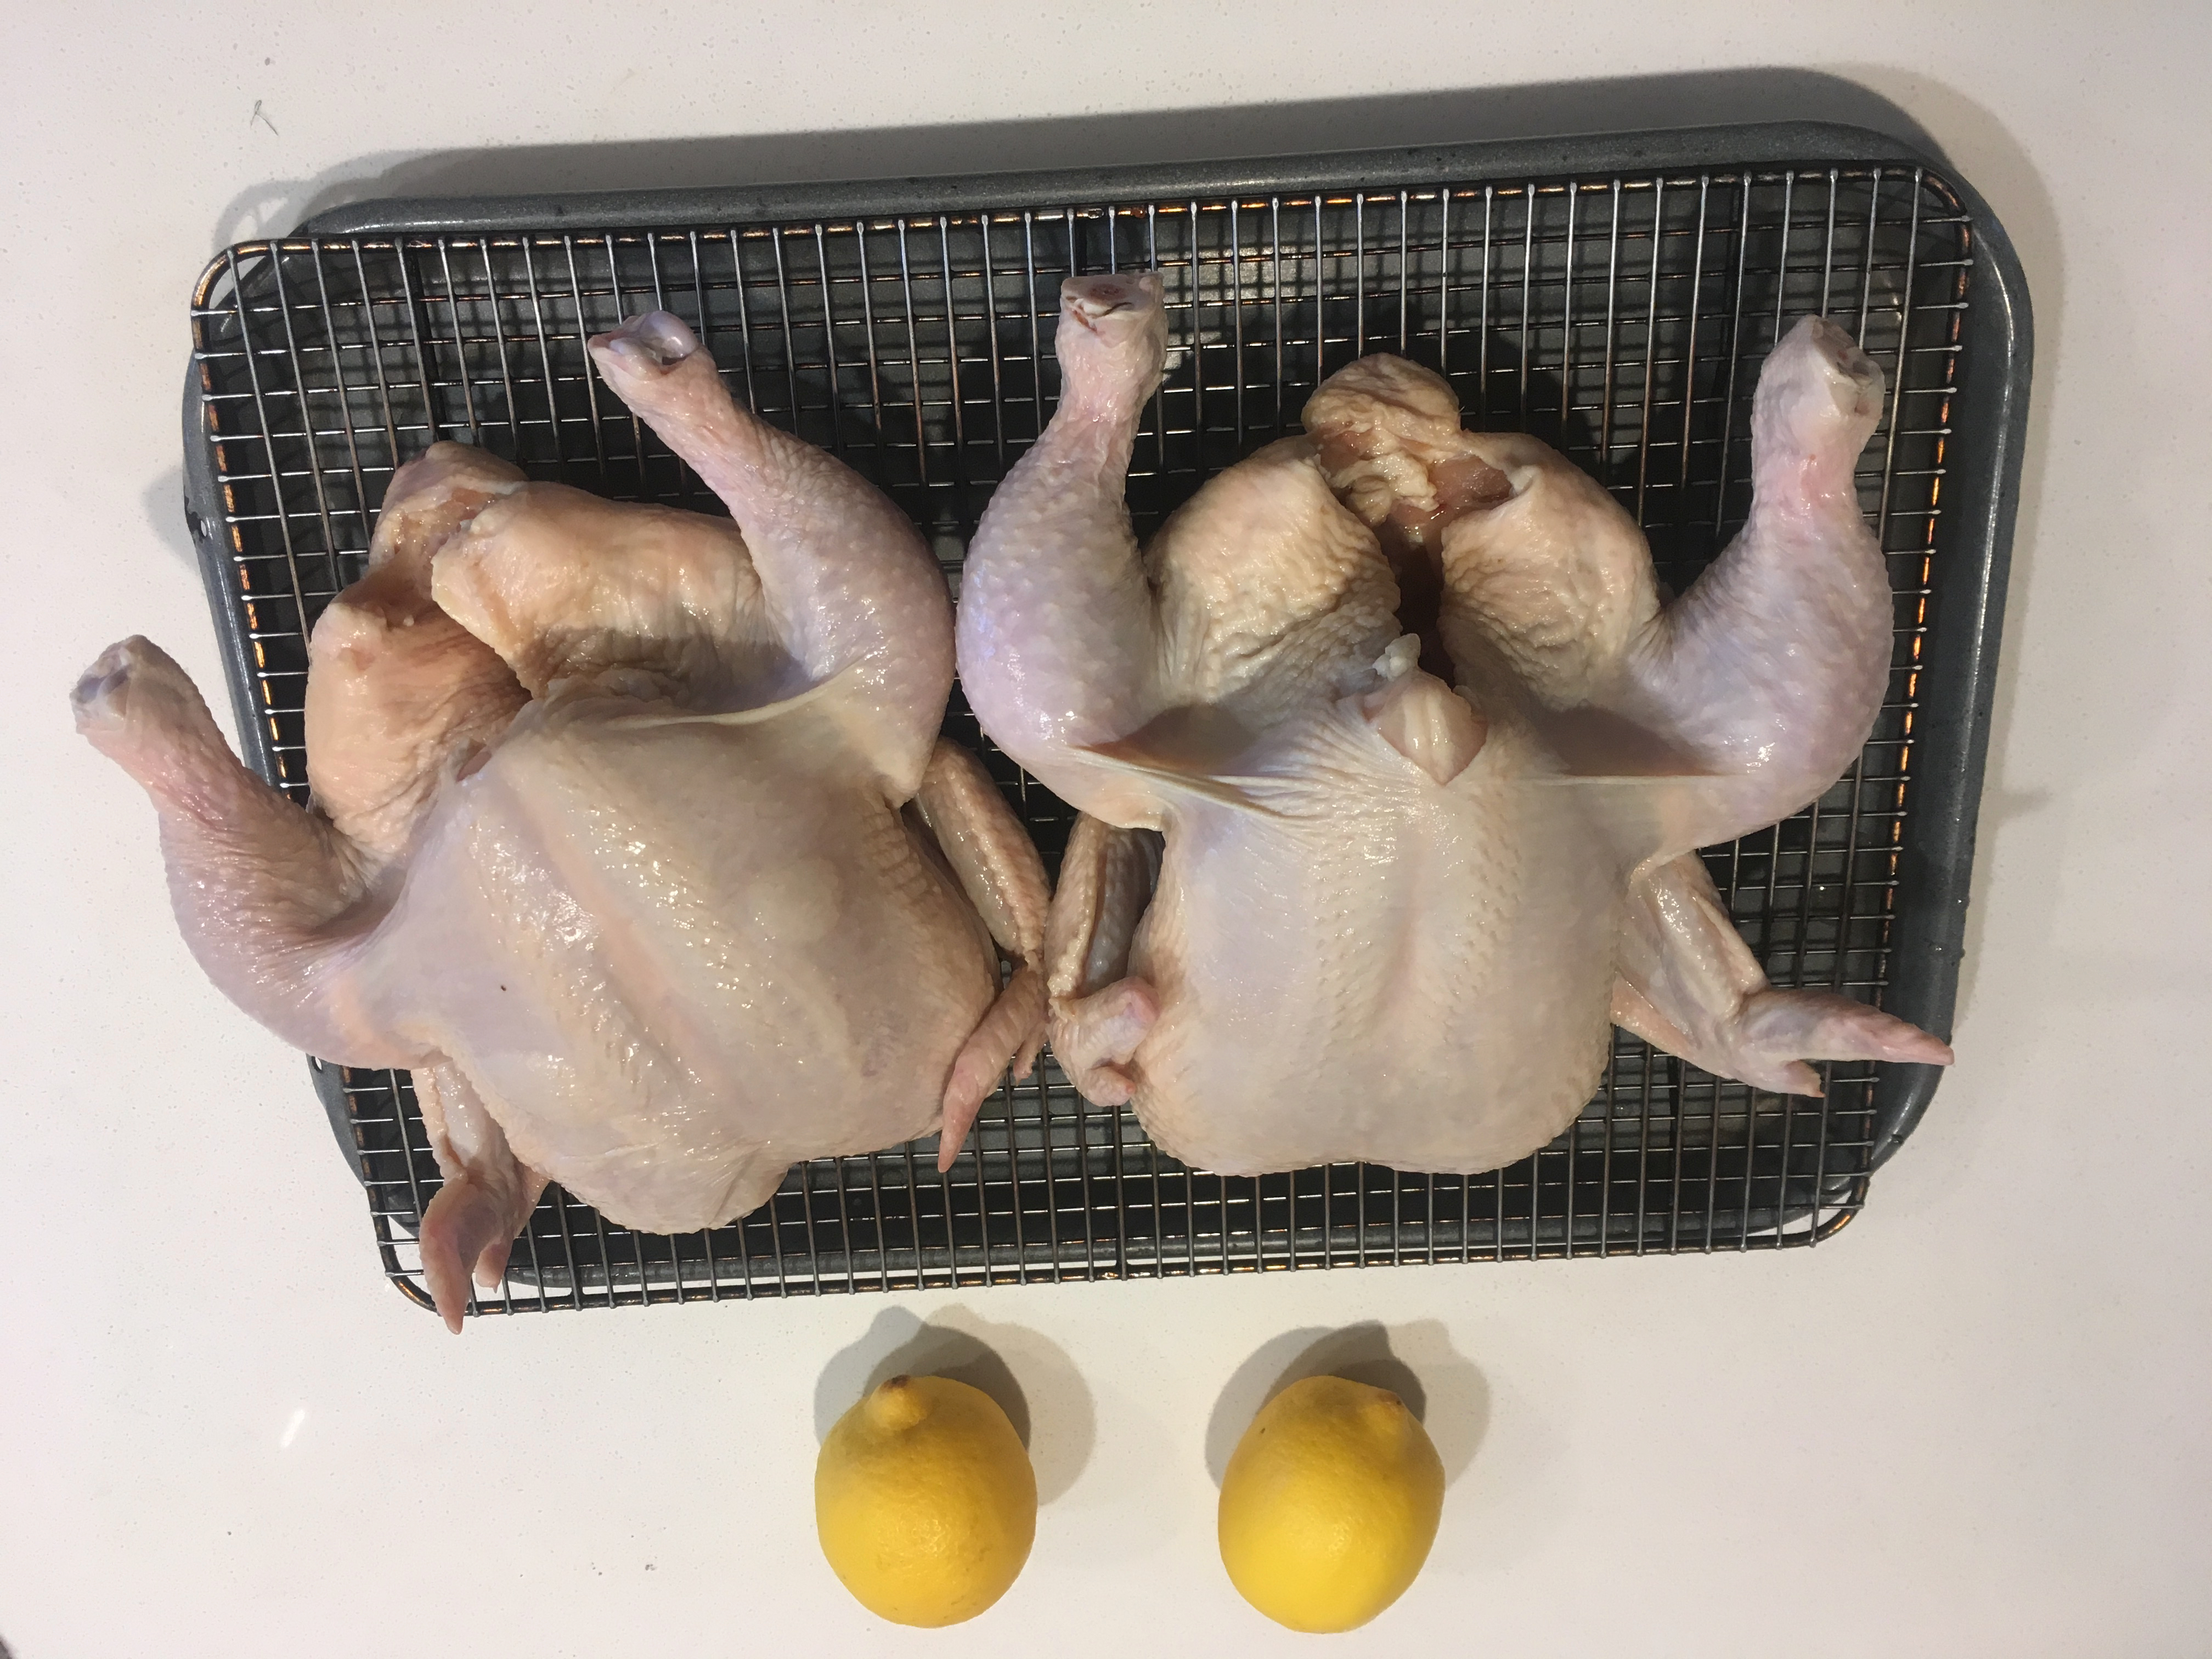
\includegraphics[width=0.25\textwidth]{\imageDir/\fileName/IMG_3197.jpg} &
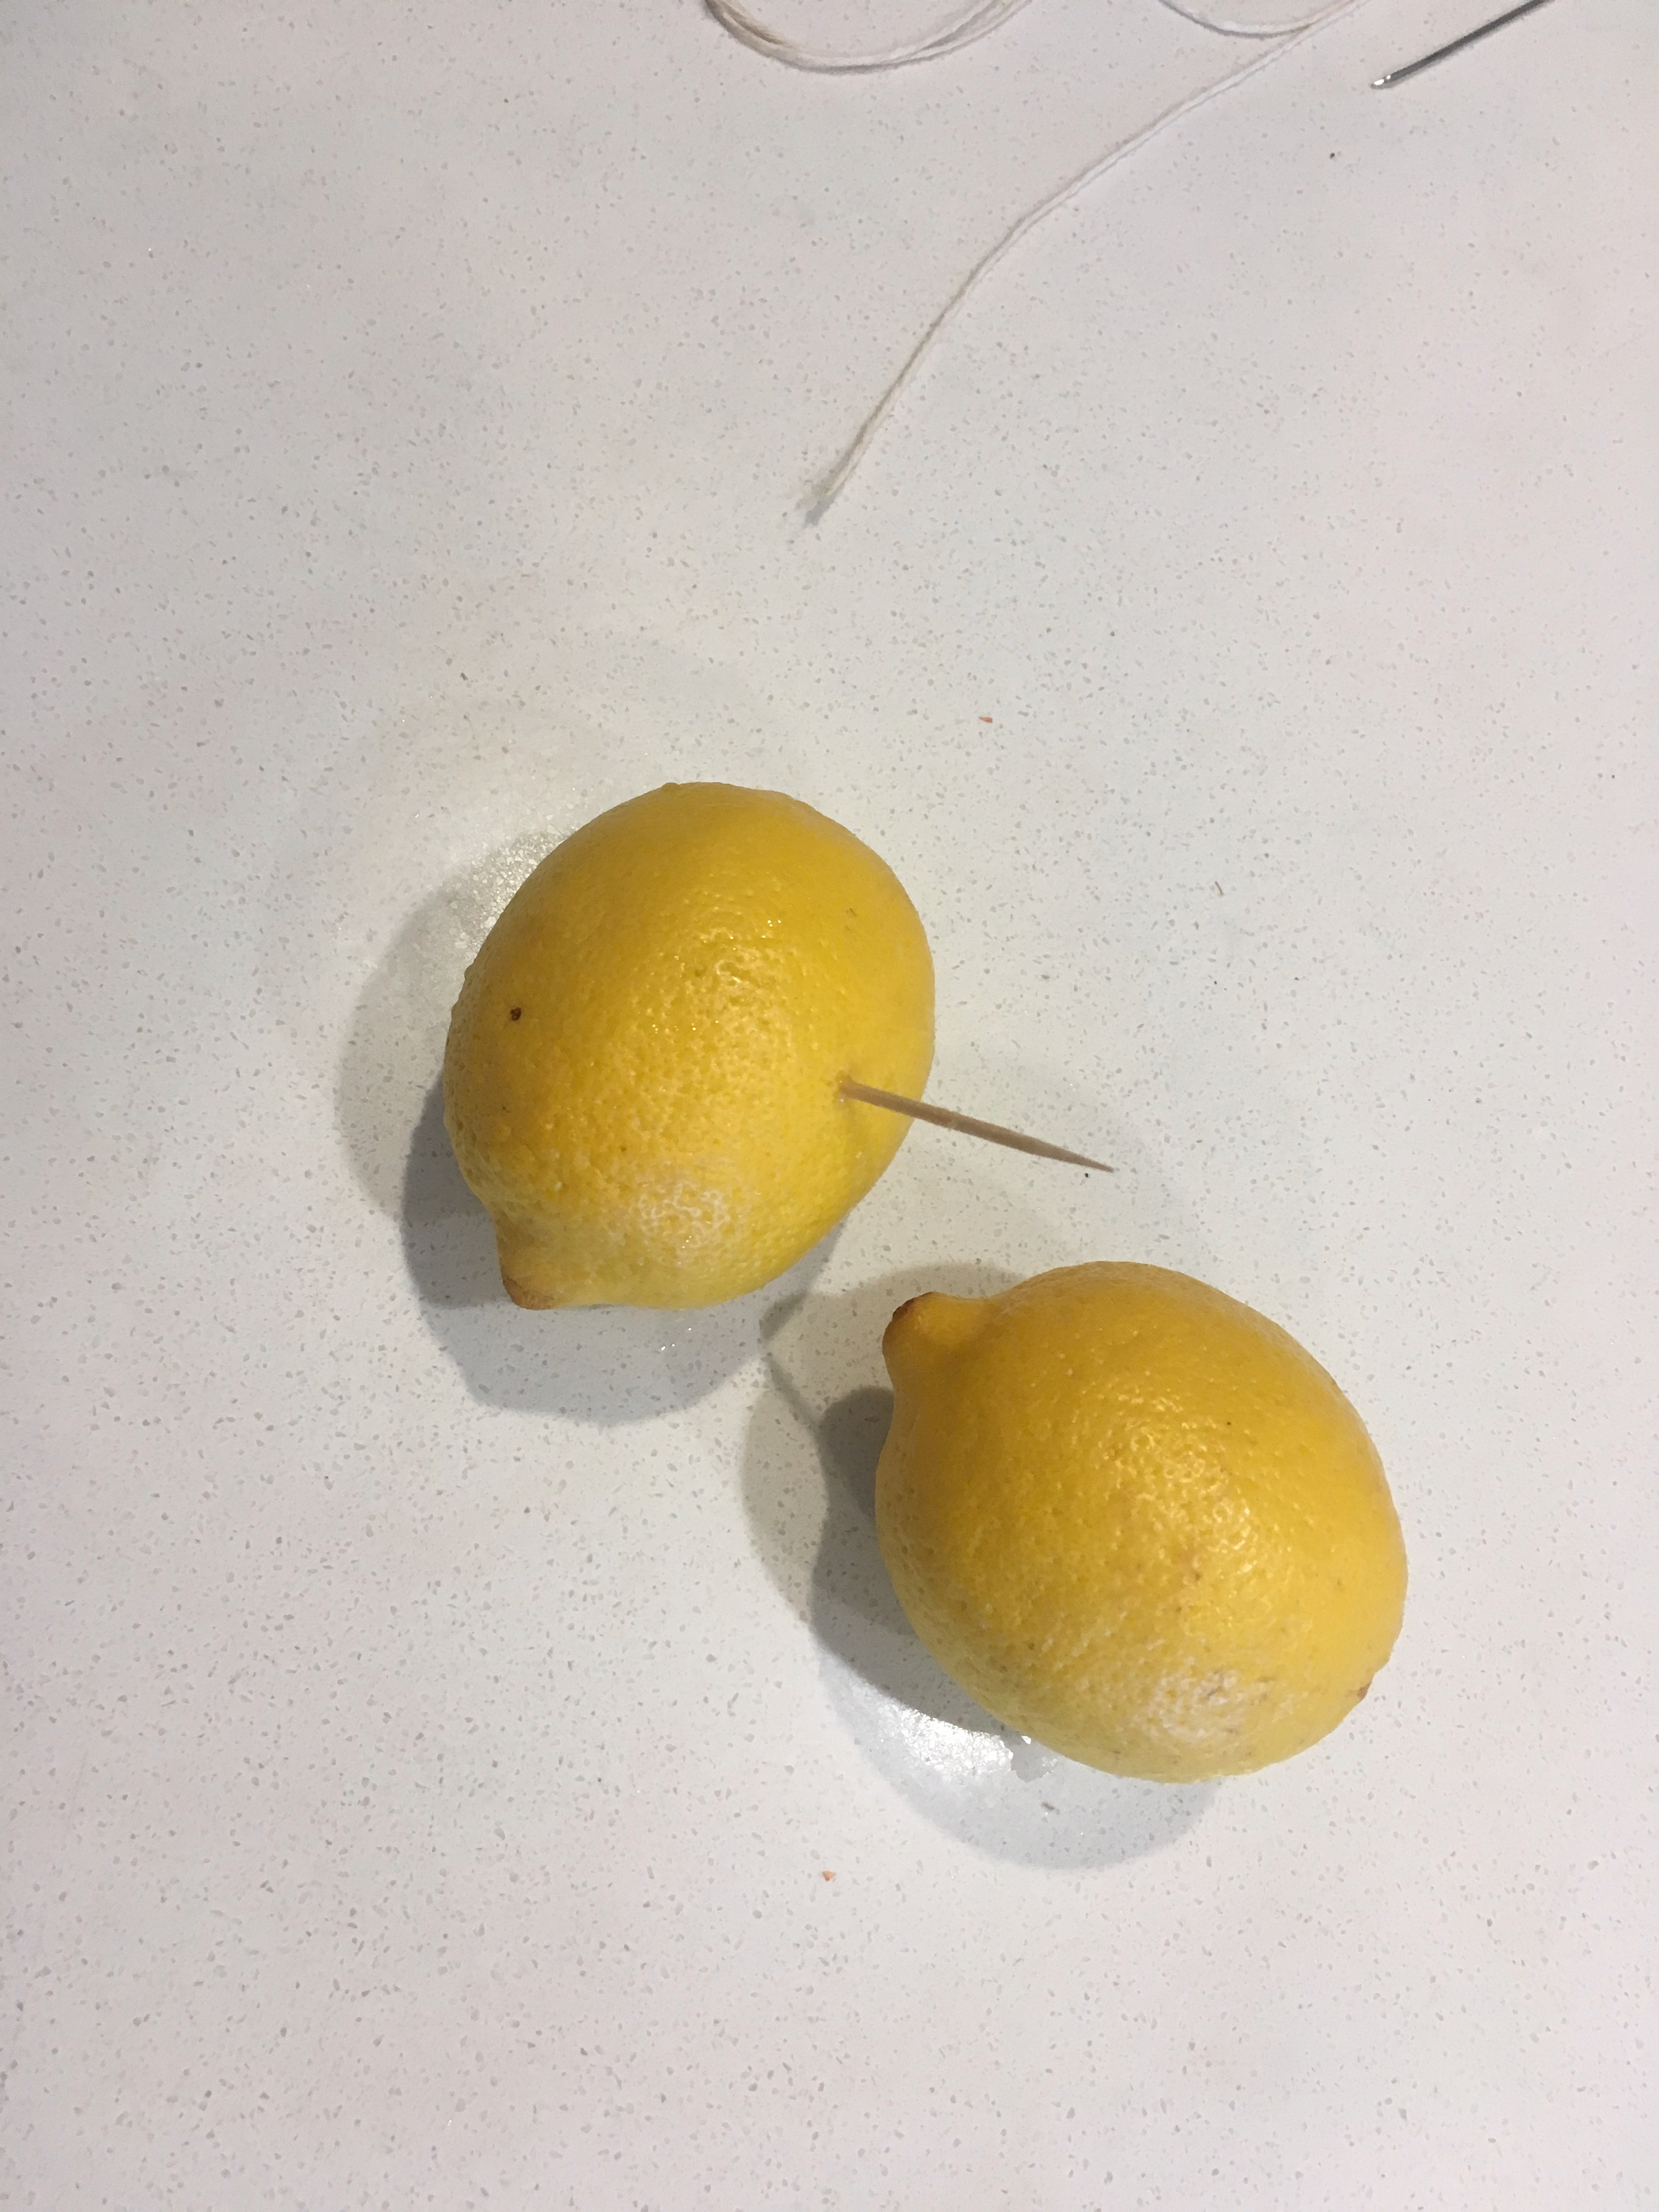
\includegraphics[width=0.25\textwidth]{\imageDir/\fileName/IMG_3212.jpg} &
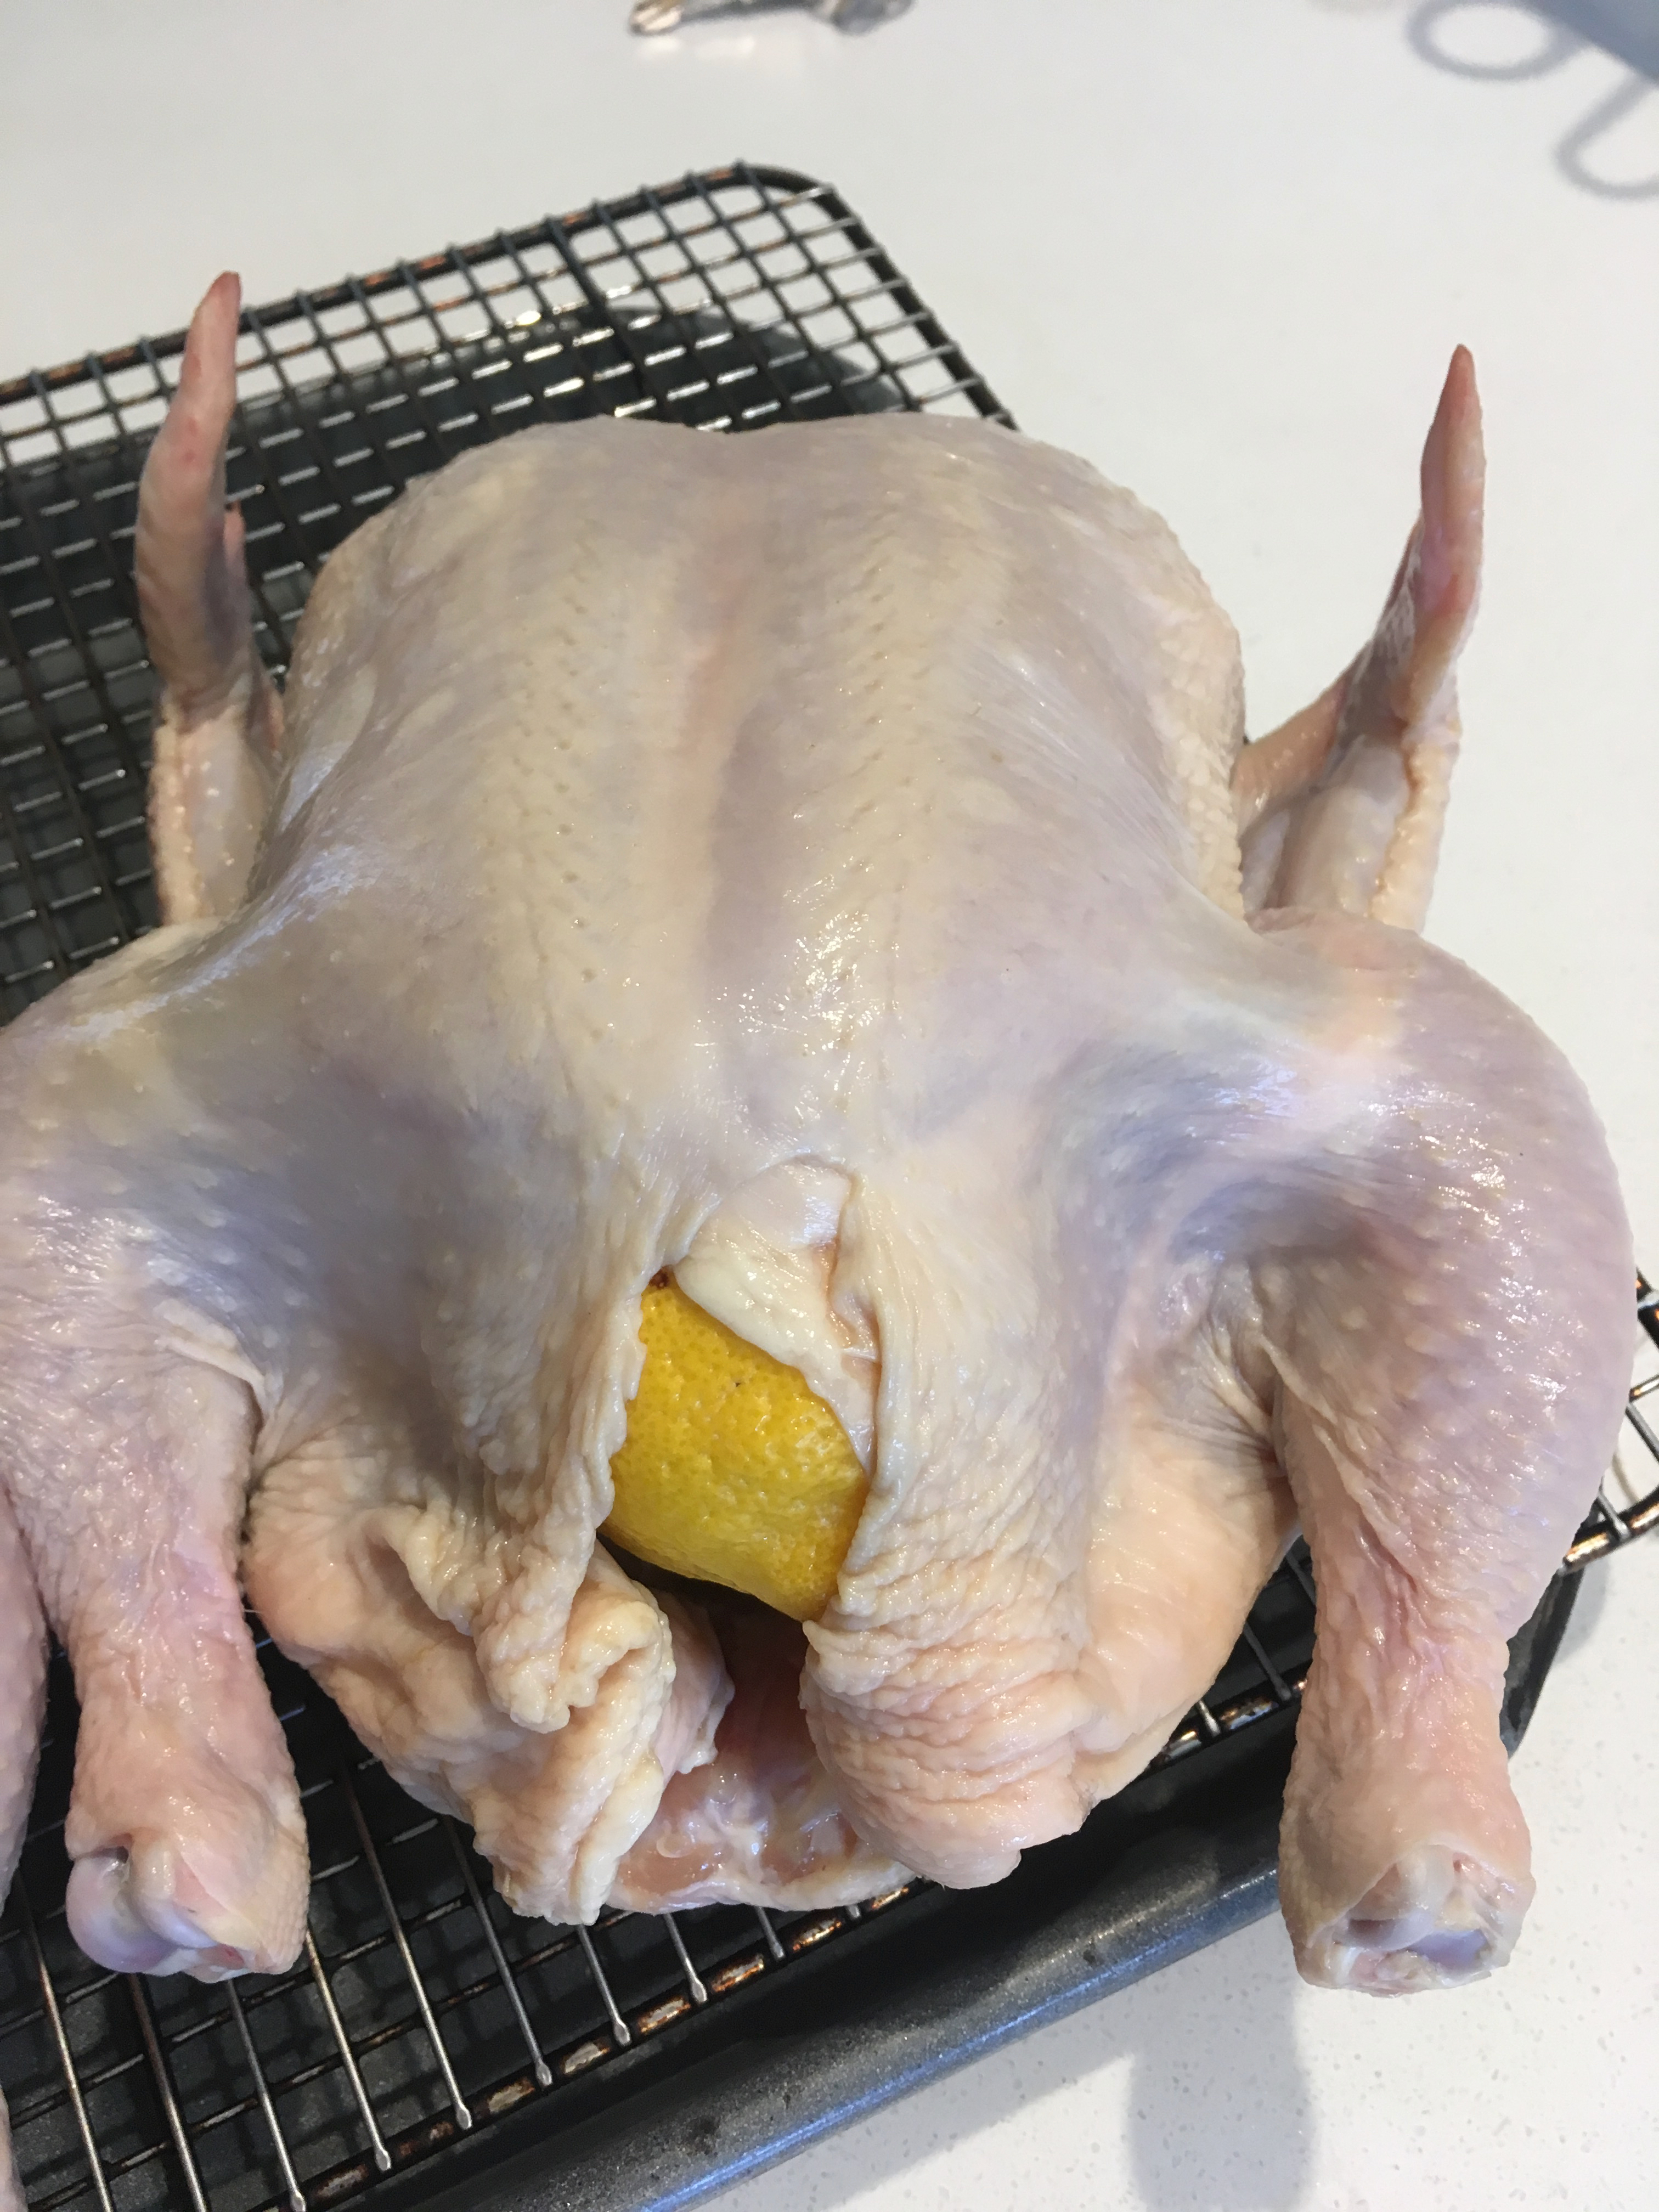
\includegraphics[width=0.25\textwidth]{\imageDir/\fileName/IMG_3213.jpg} \\
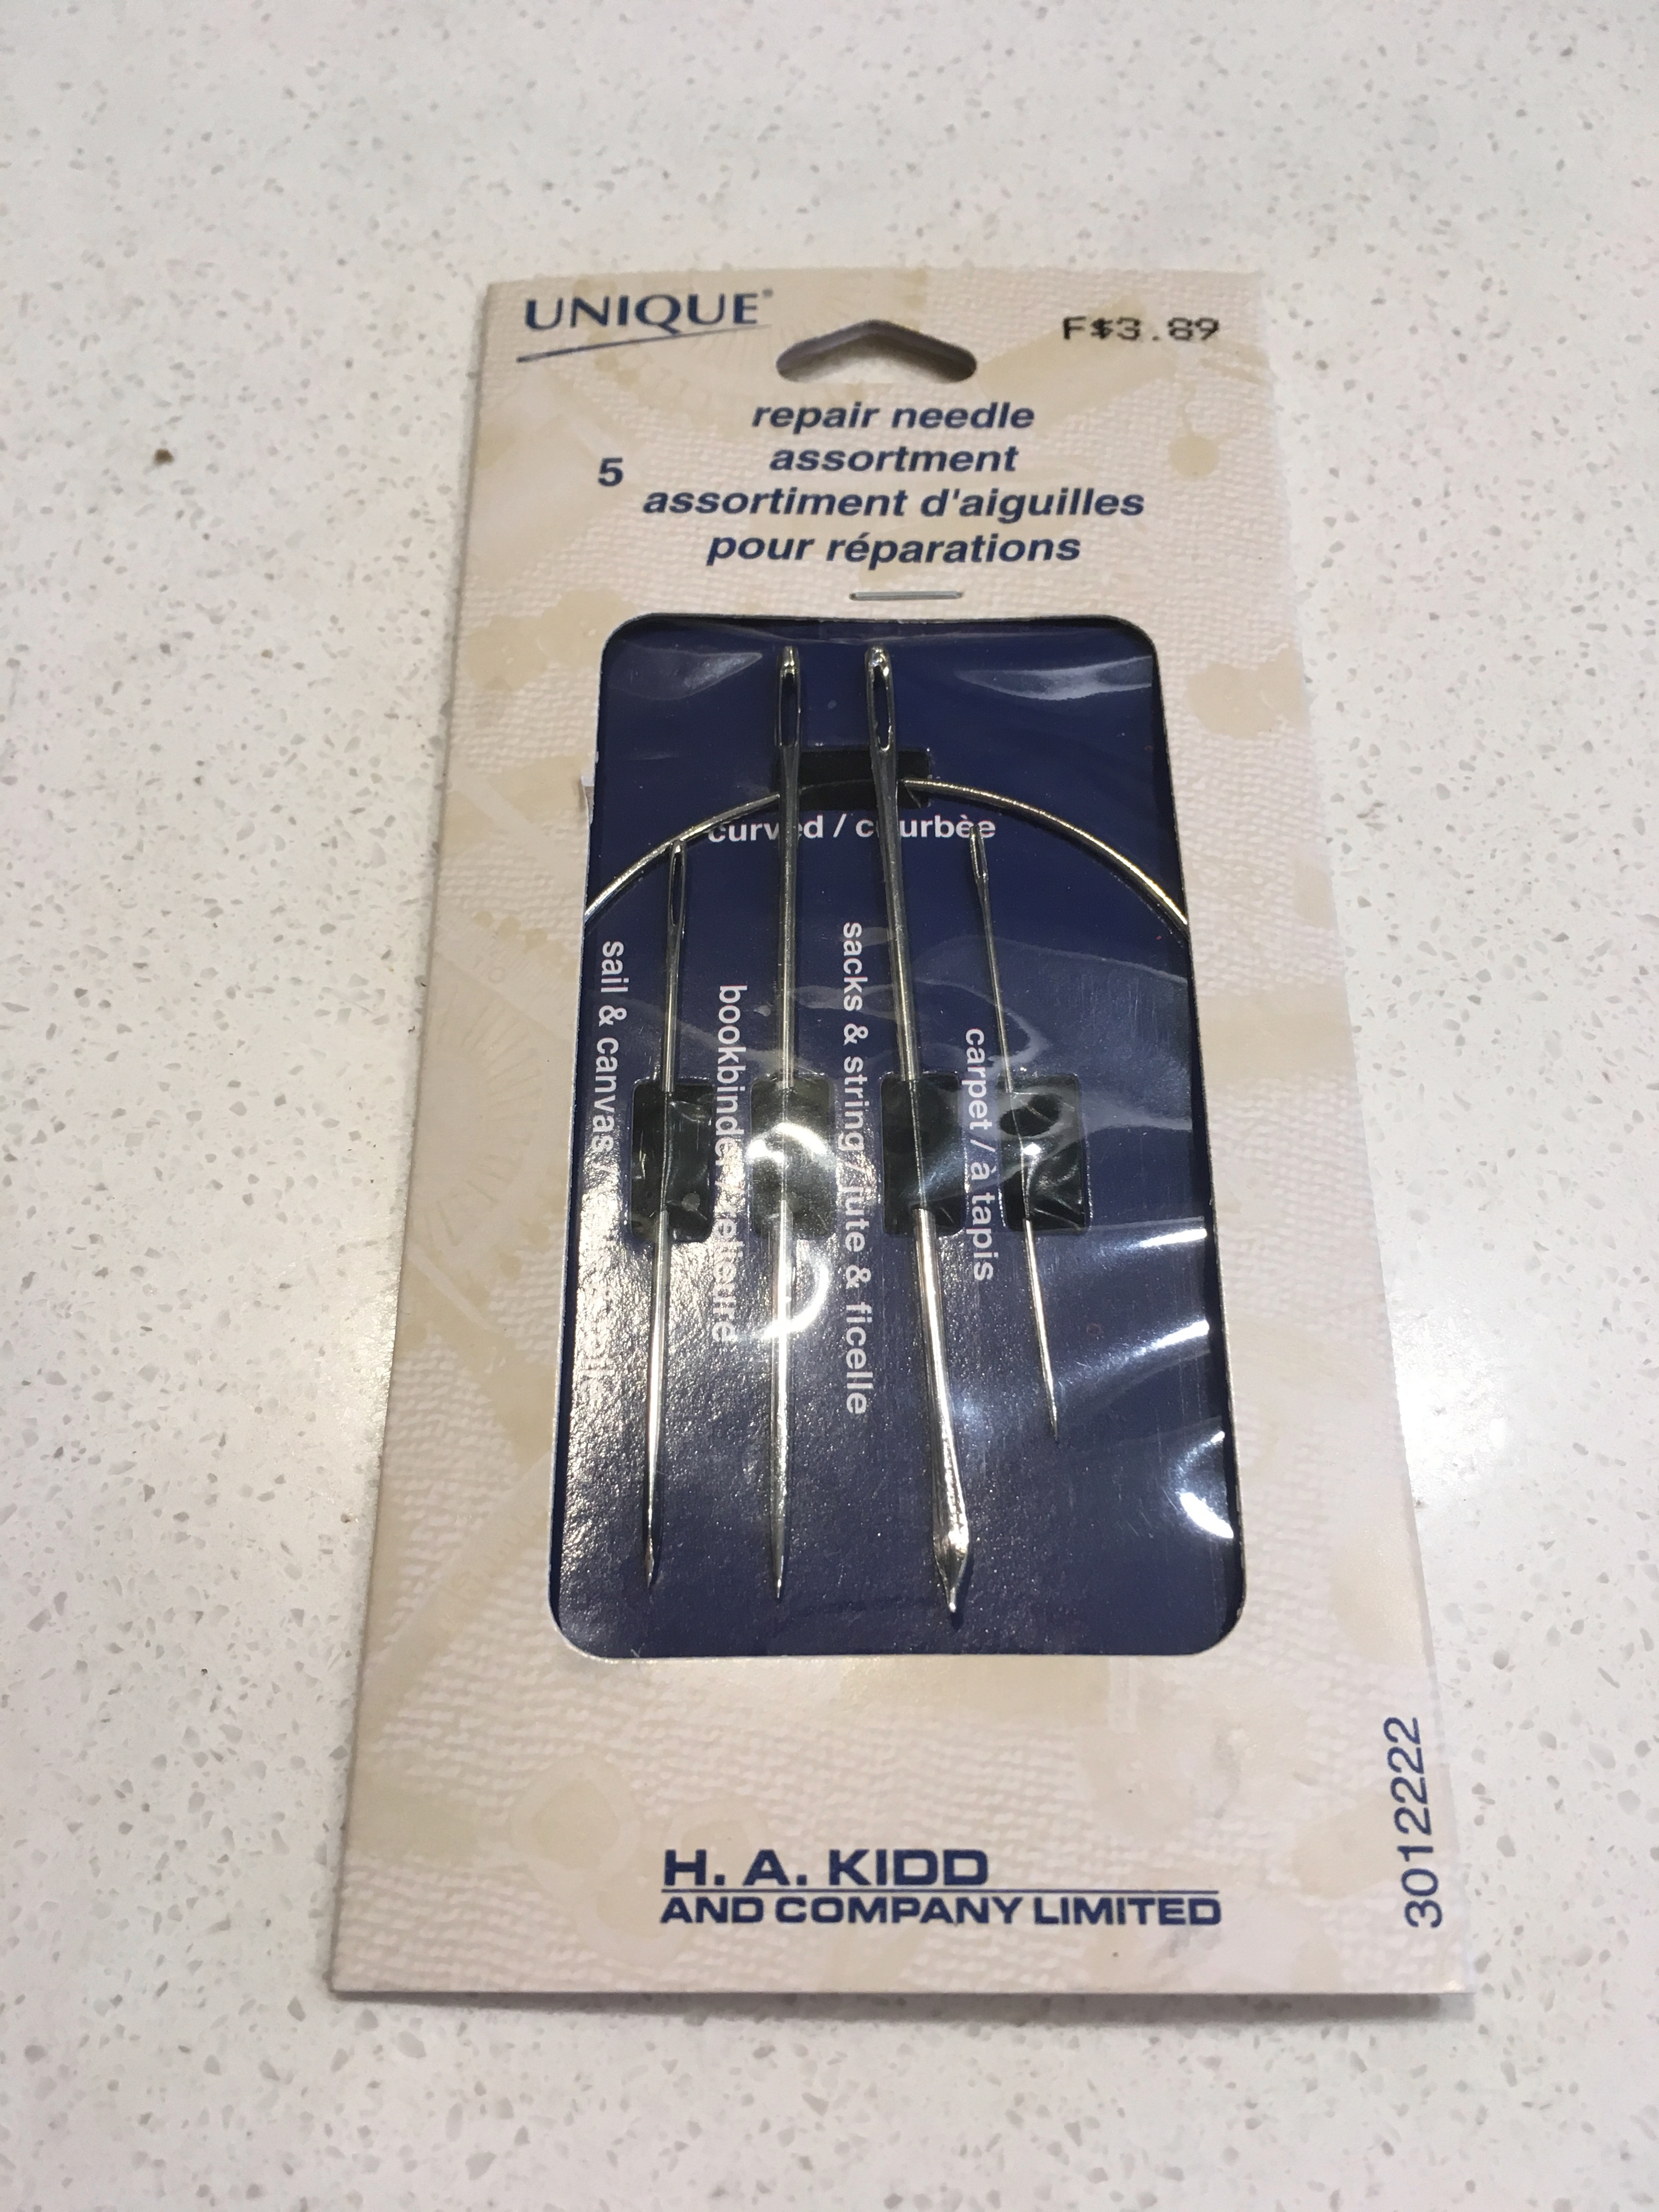
\includegraphics[width=0.25\textwidth]{\imageDir/\fileName/IMG_3206.jpg} &
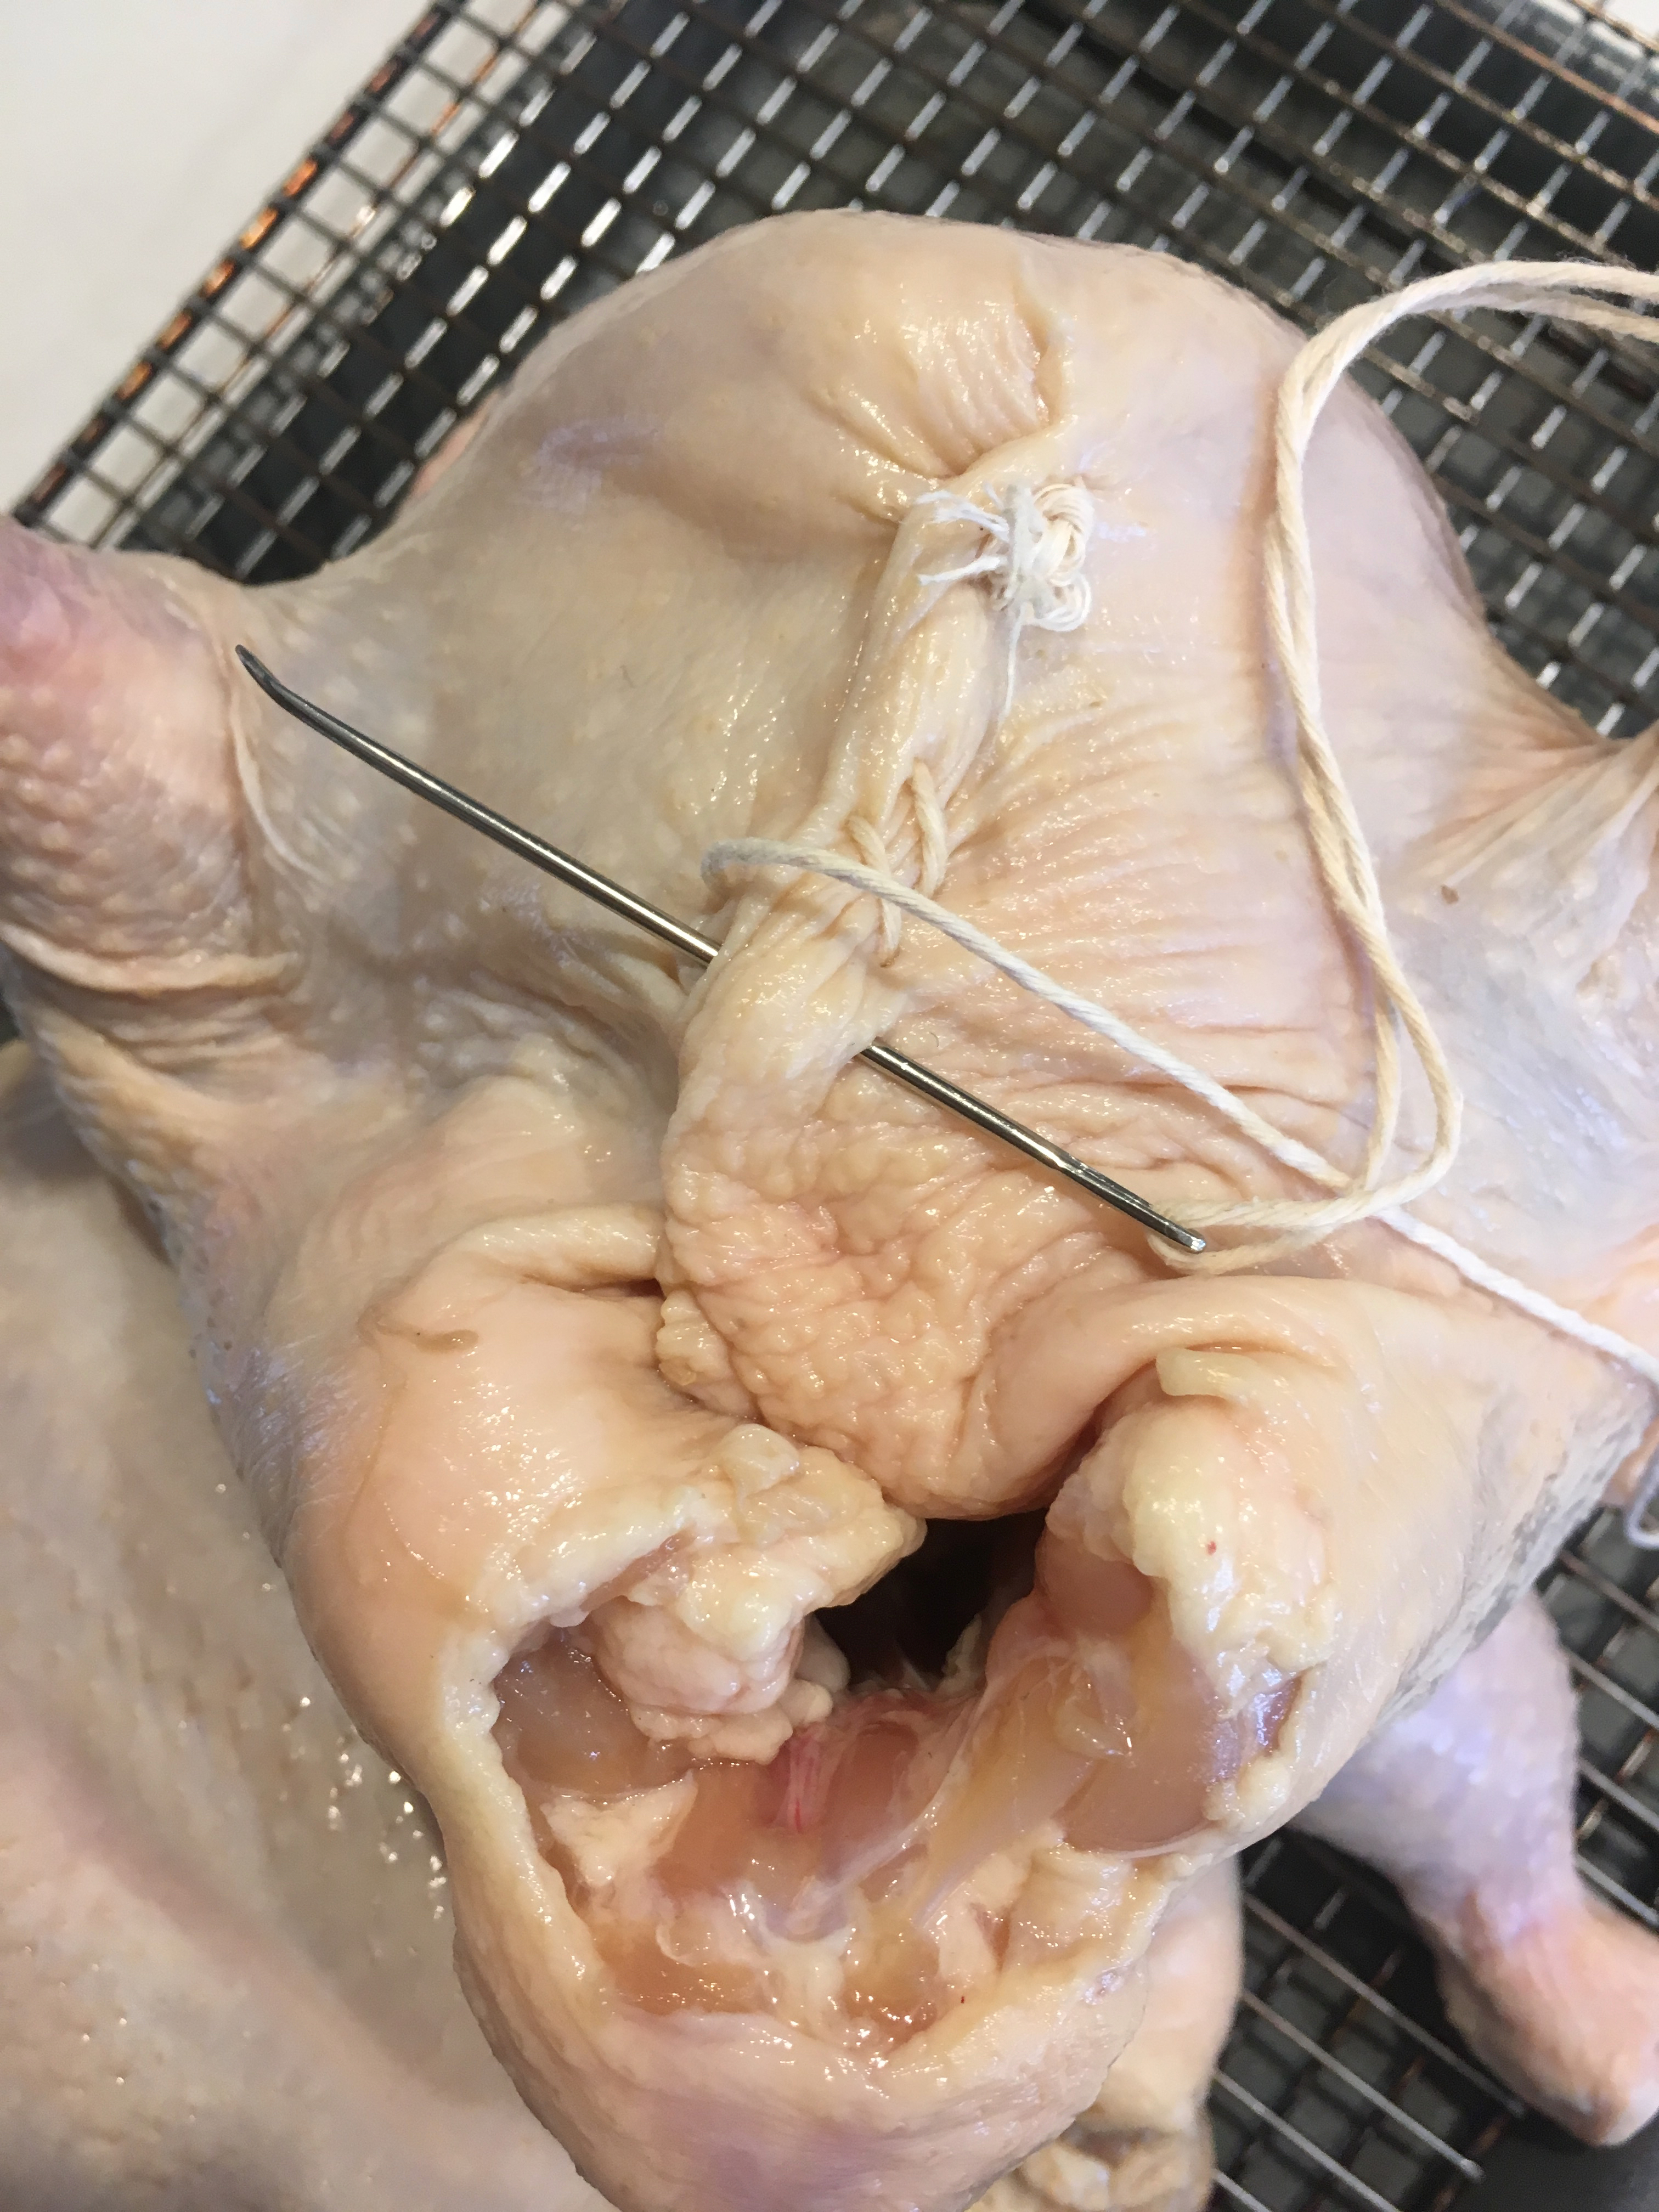
\includegraphics[width=0.25\textwidth]{\imageDir/\fileName/IMG_3214.jpg} &
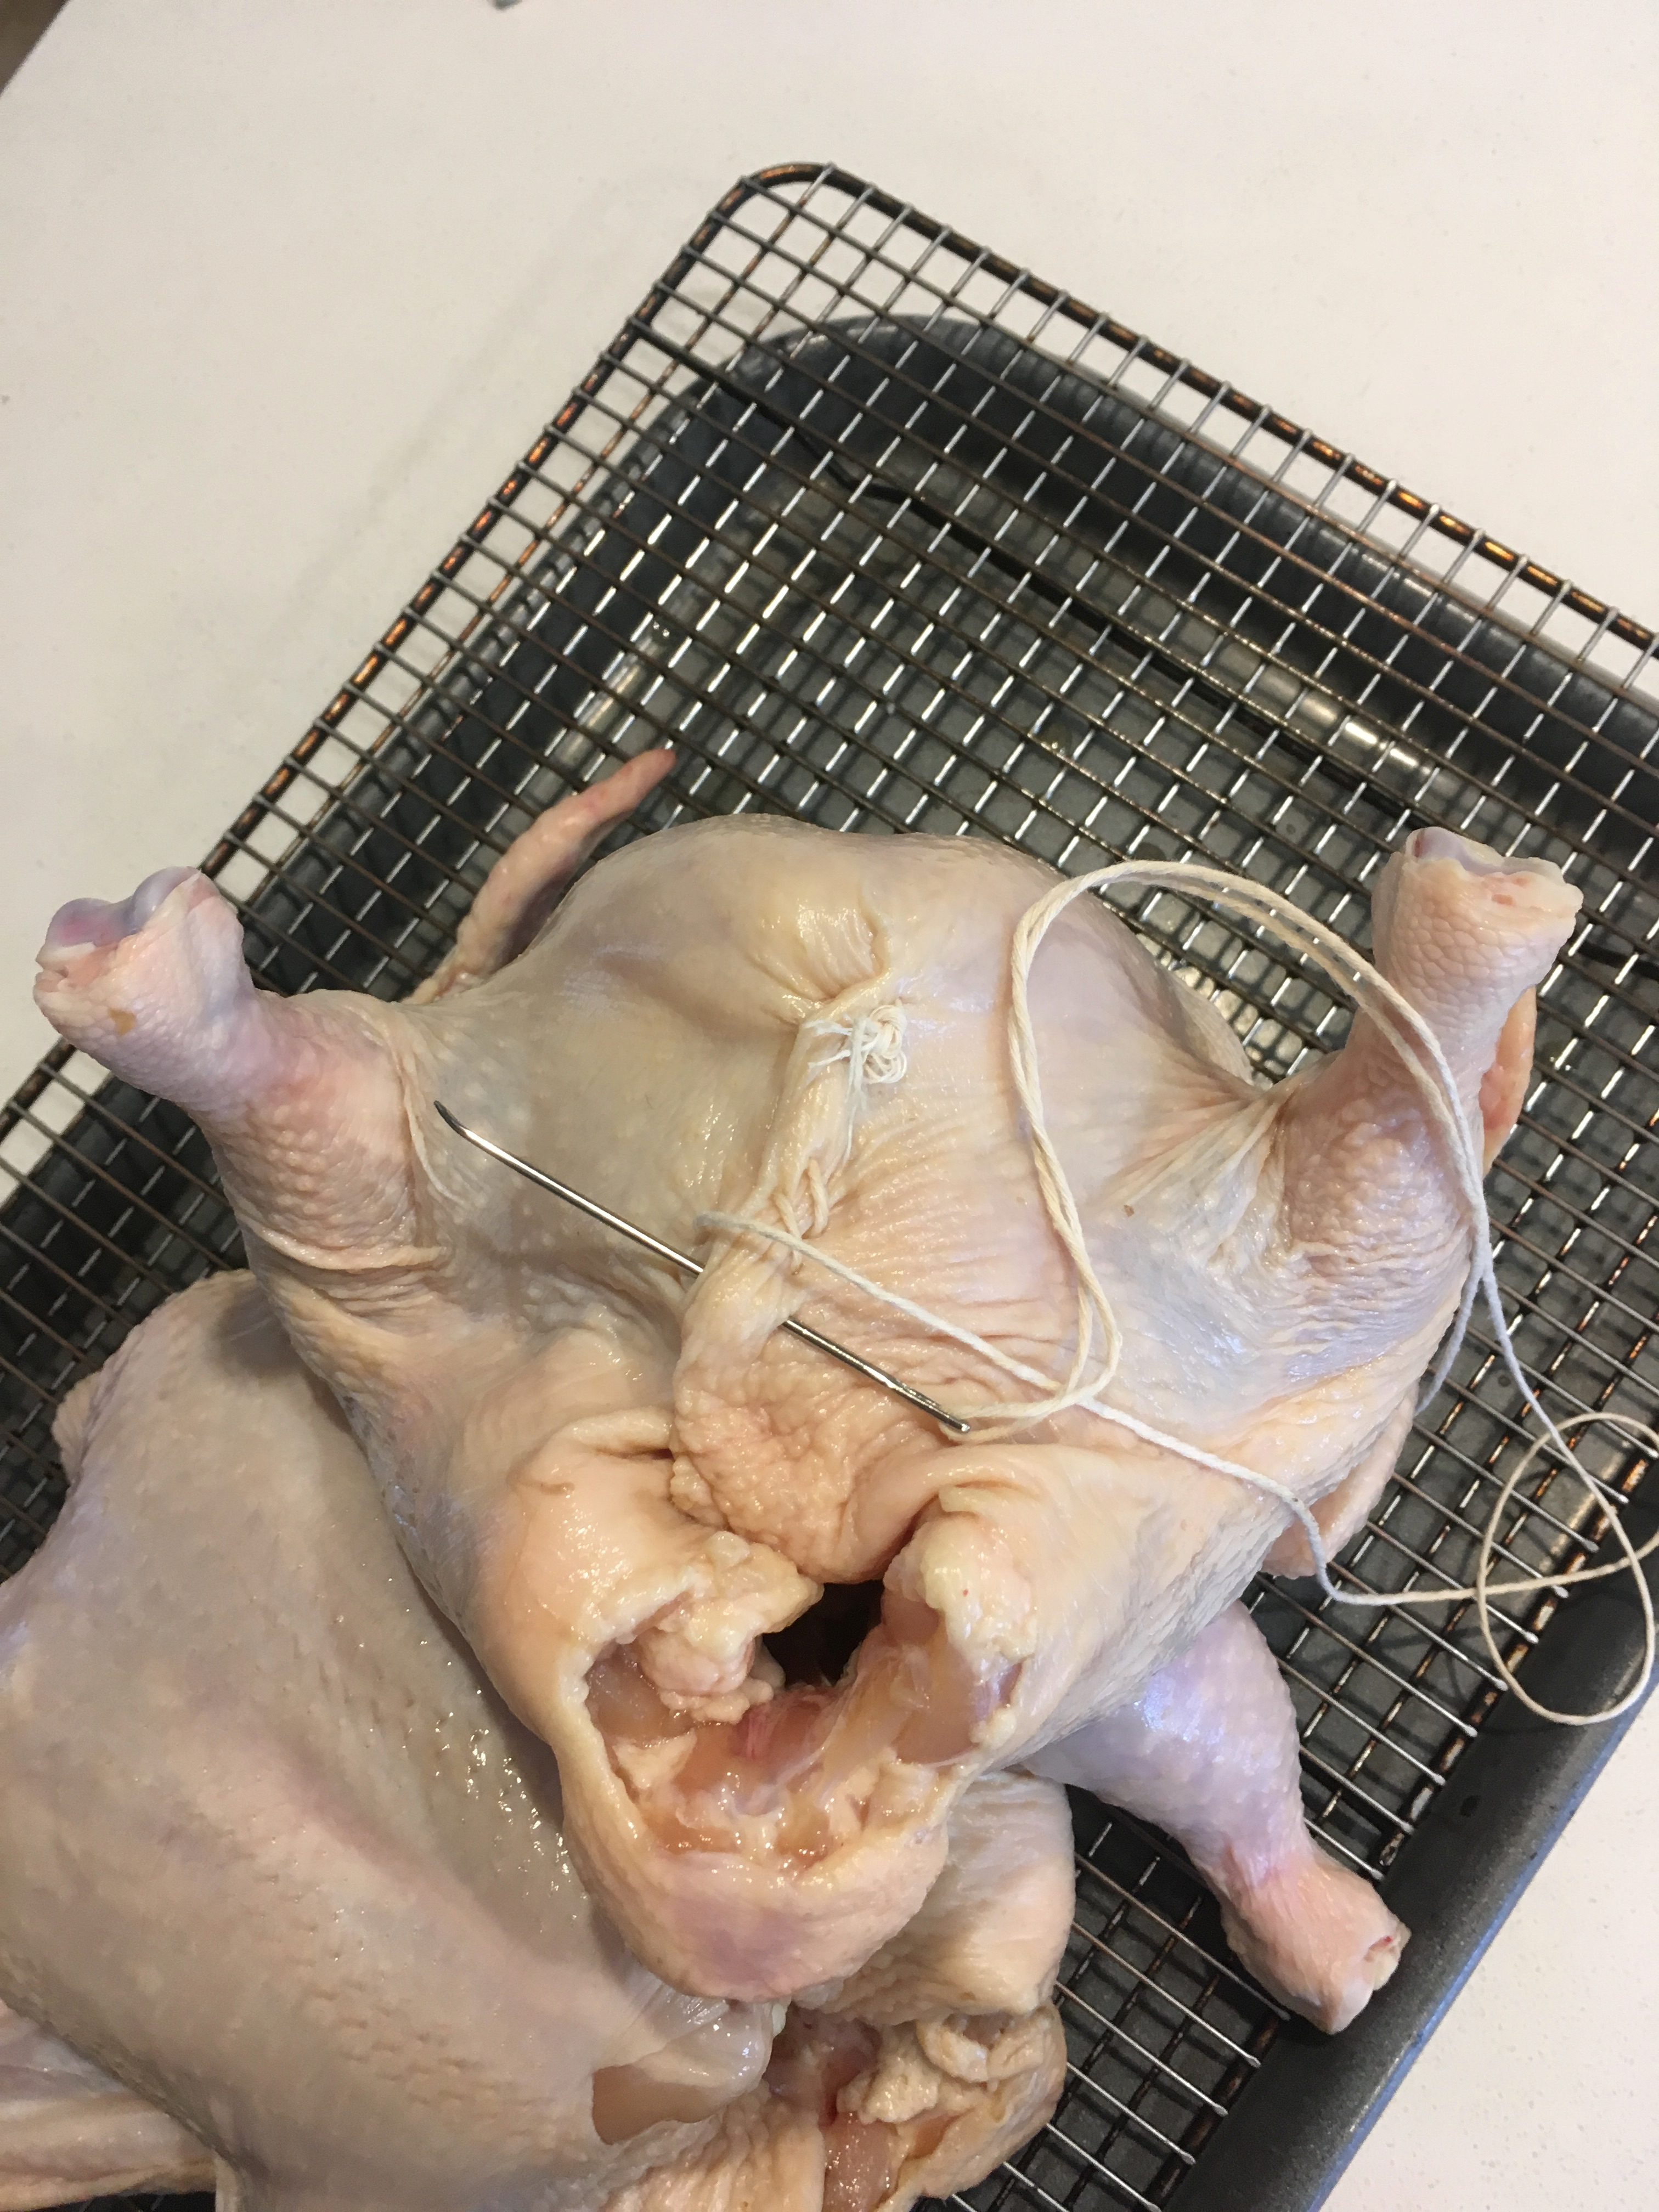
\includegraphics[width=0.25\textwidth]{\imageDir/\fileName/IMG_3216.jpg} \\
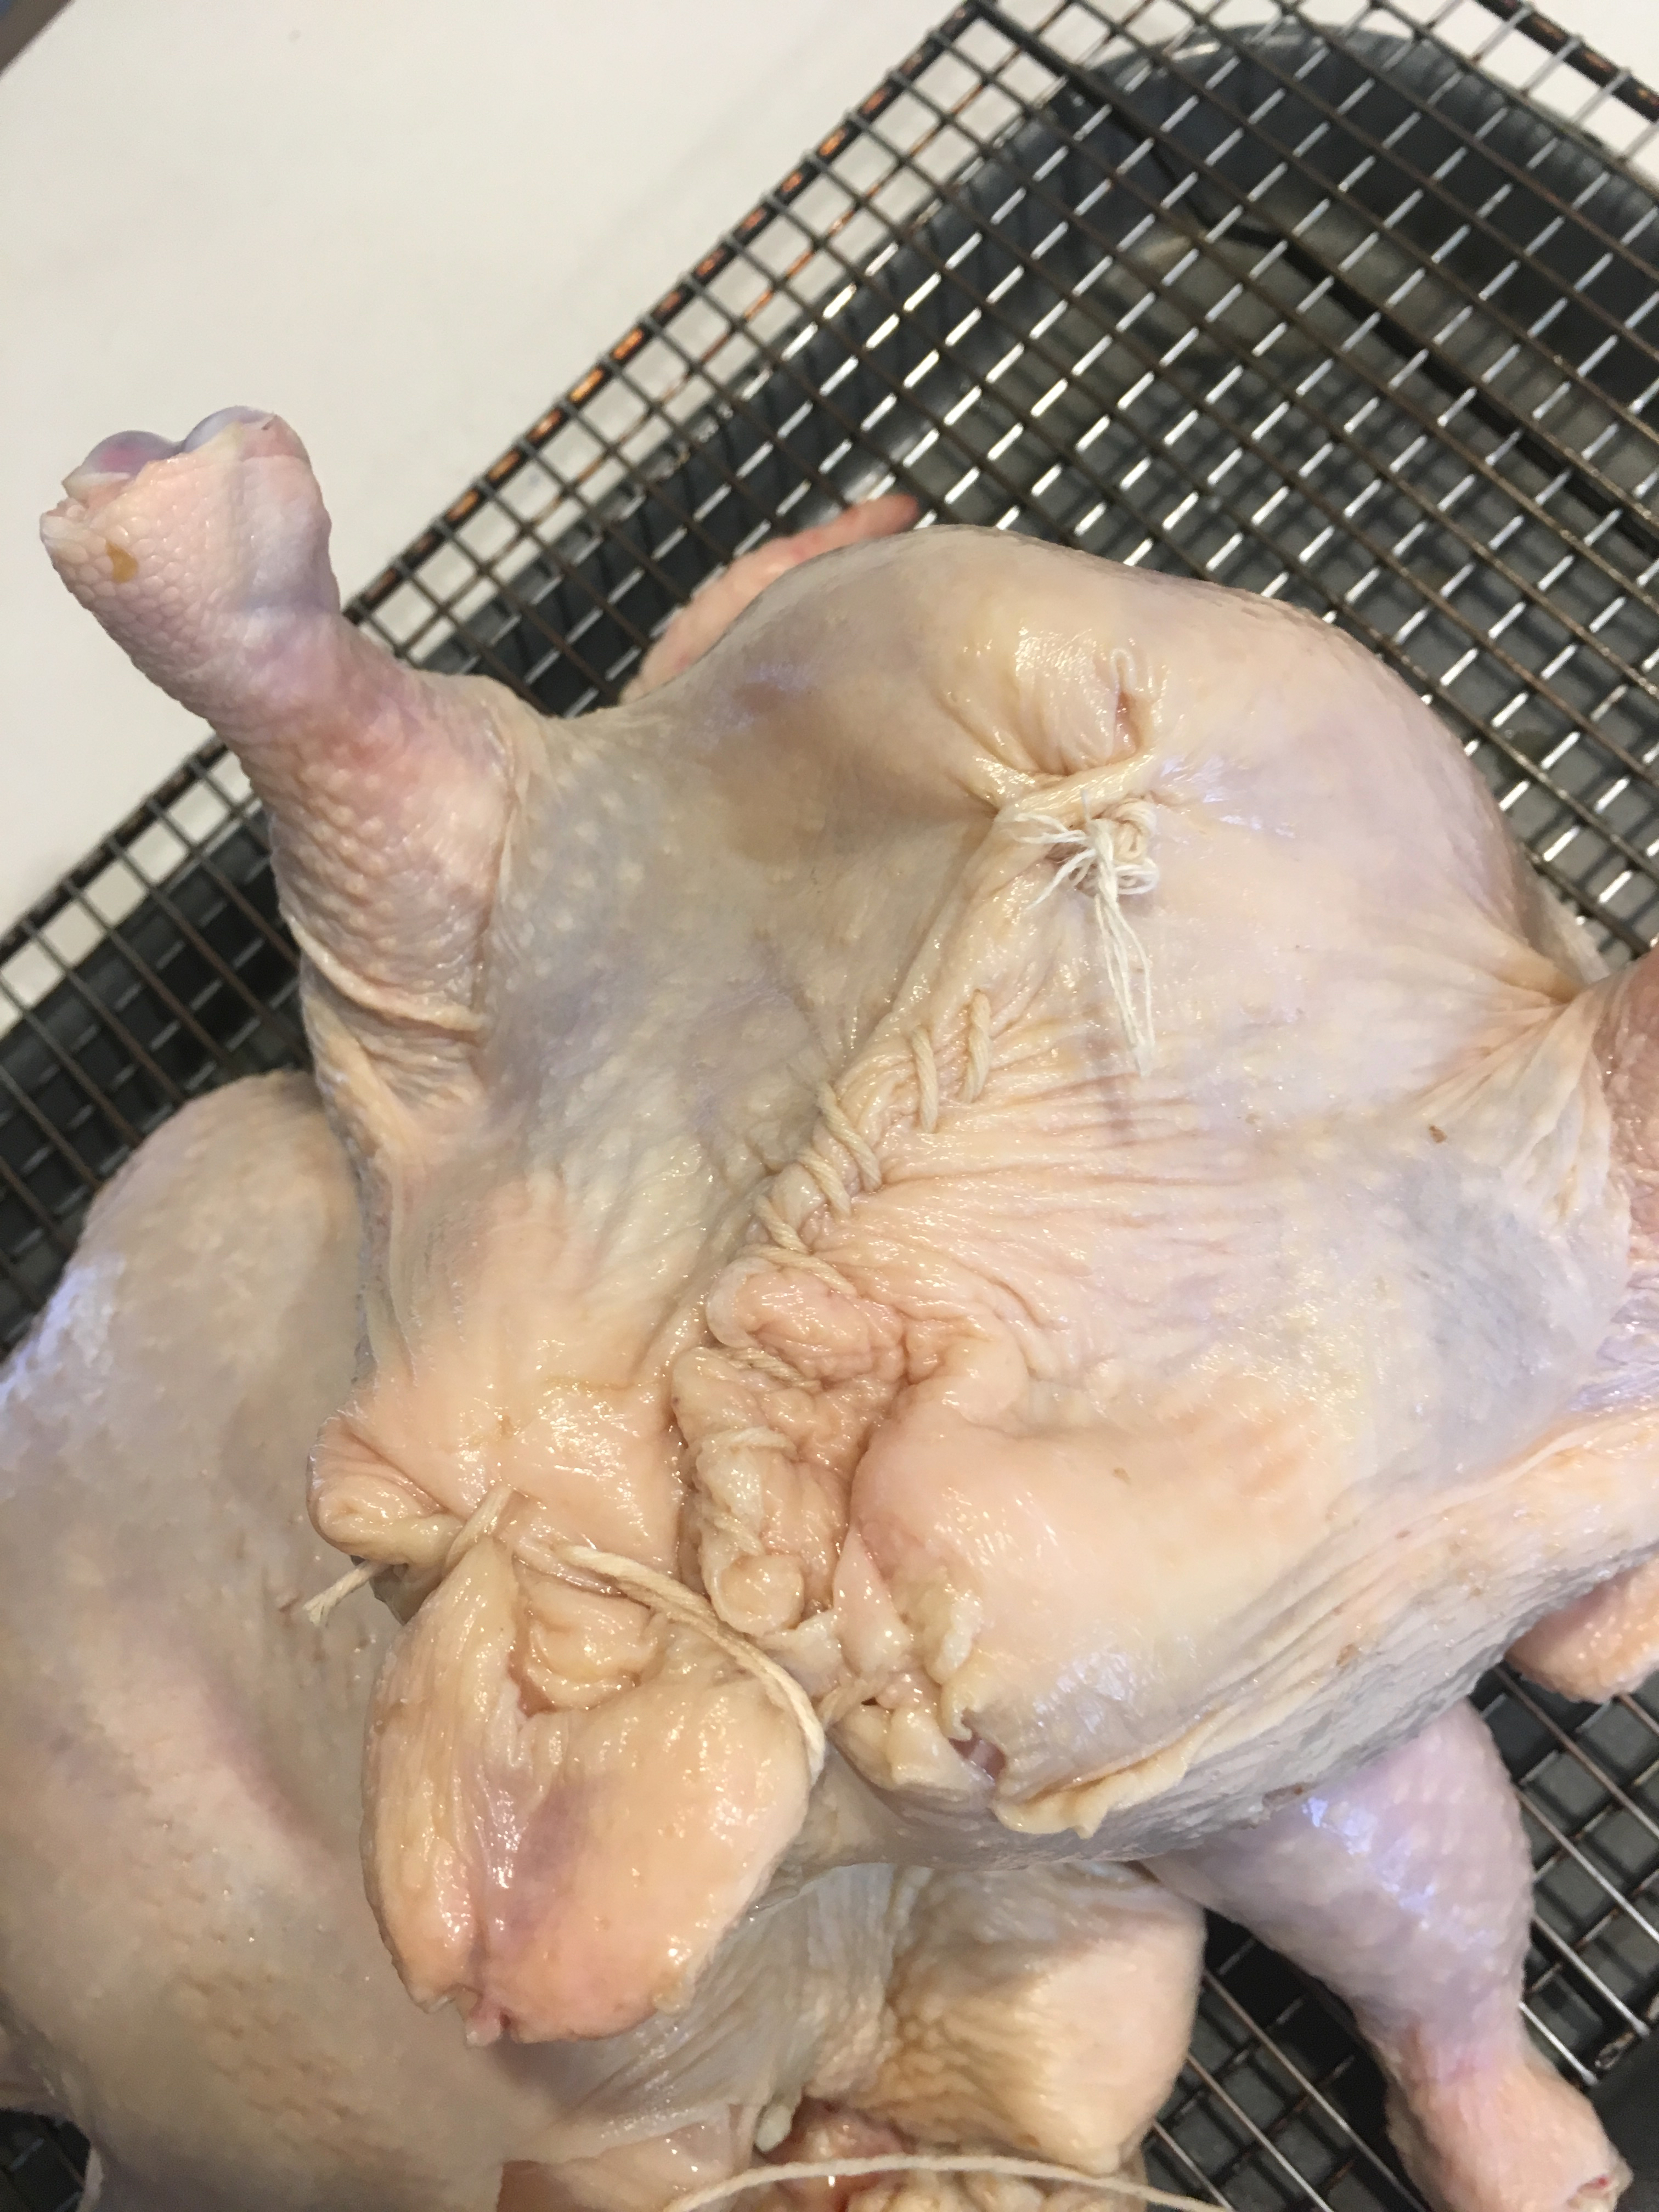
\includegraphics[width=0.25\textwidth]{\imageDir/\fileName/IMG_3217.jpg} &
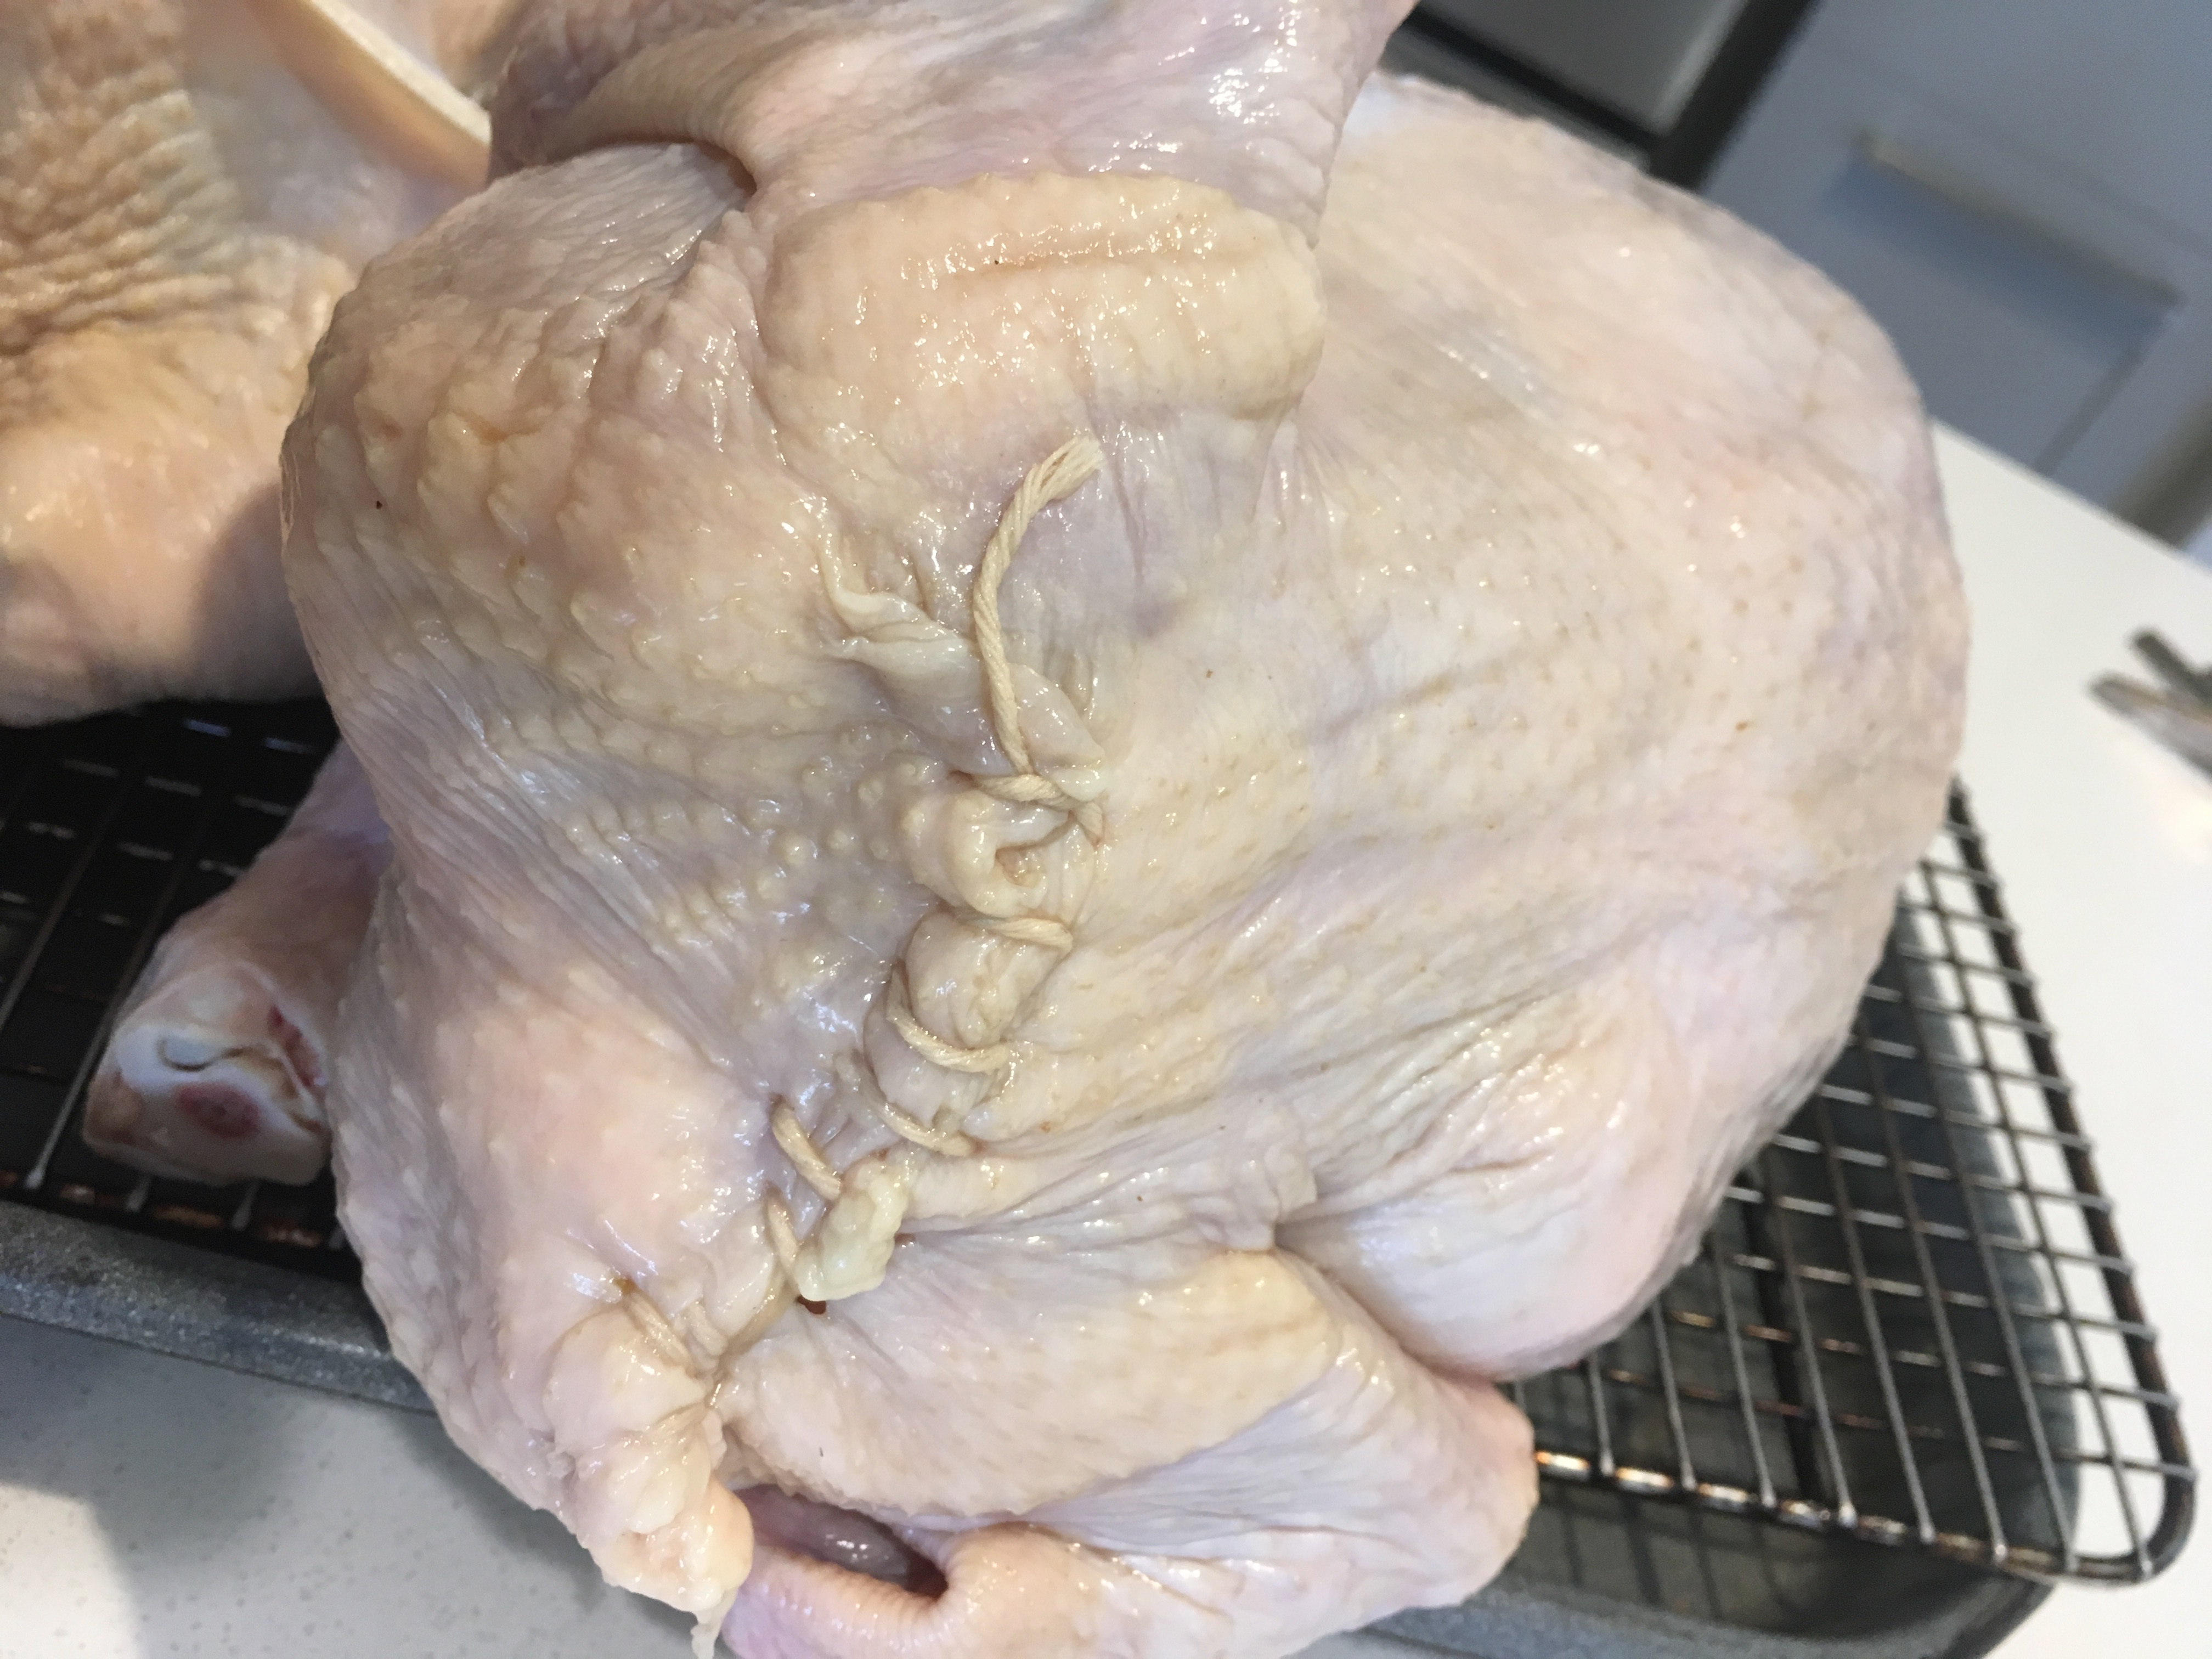
\includegraphics[width=0.25\textwidth]{\imageDir/\fileName/IMG_3218.jpg} &
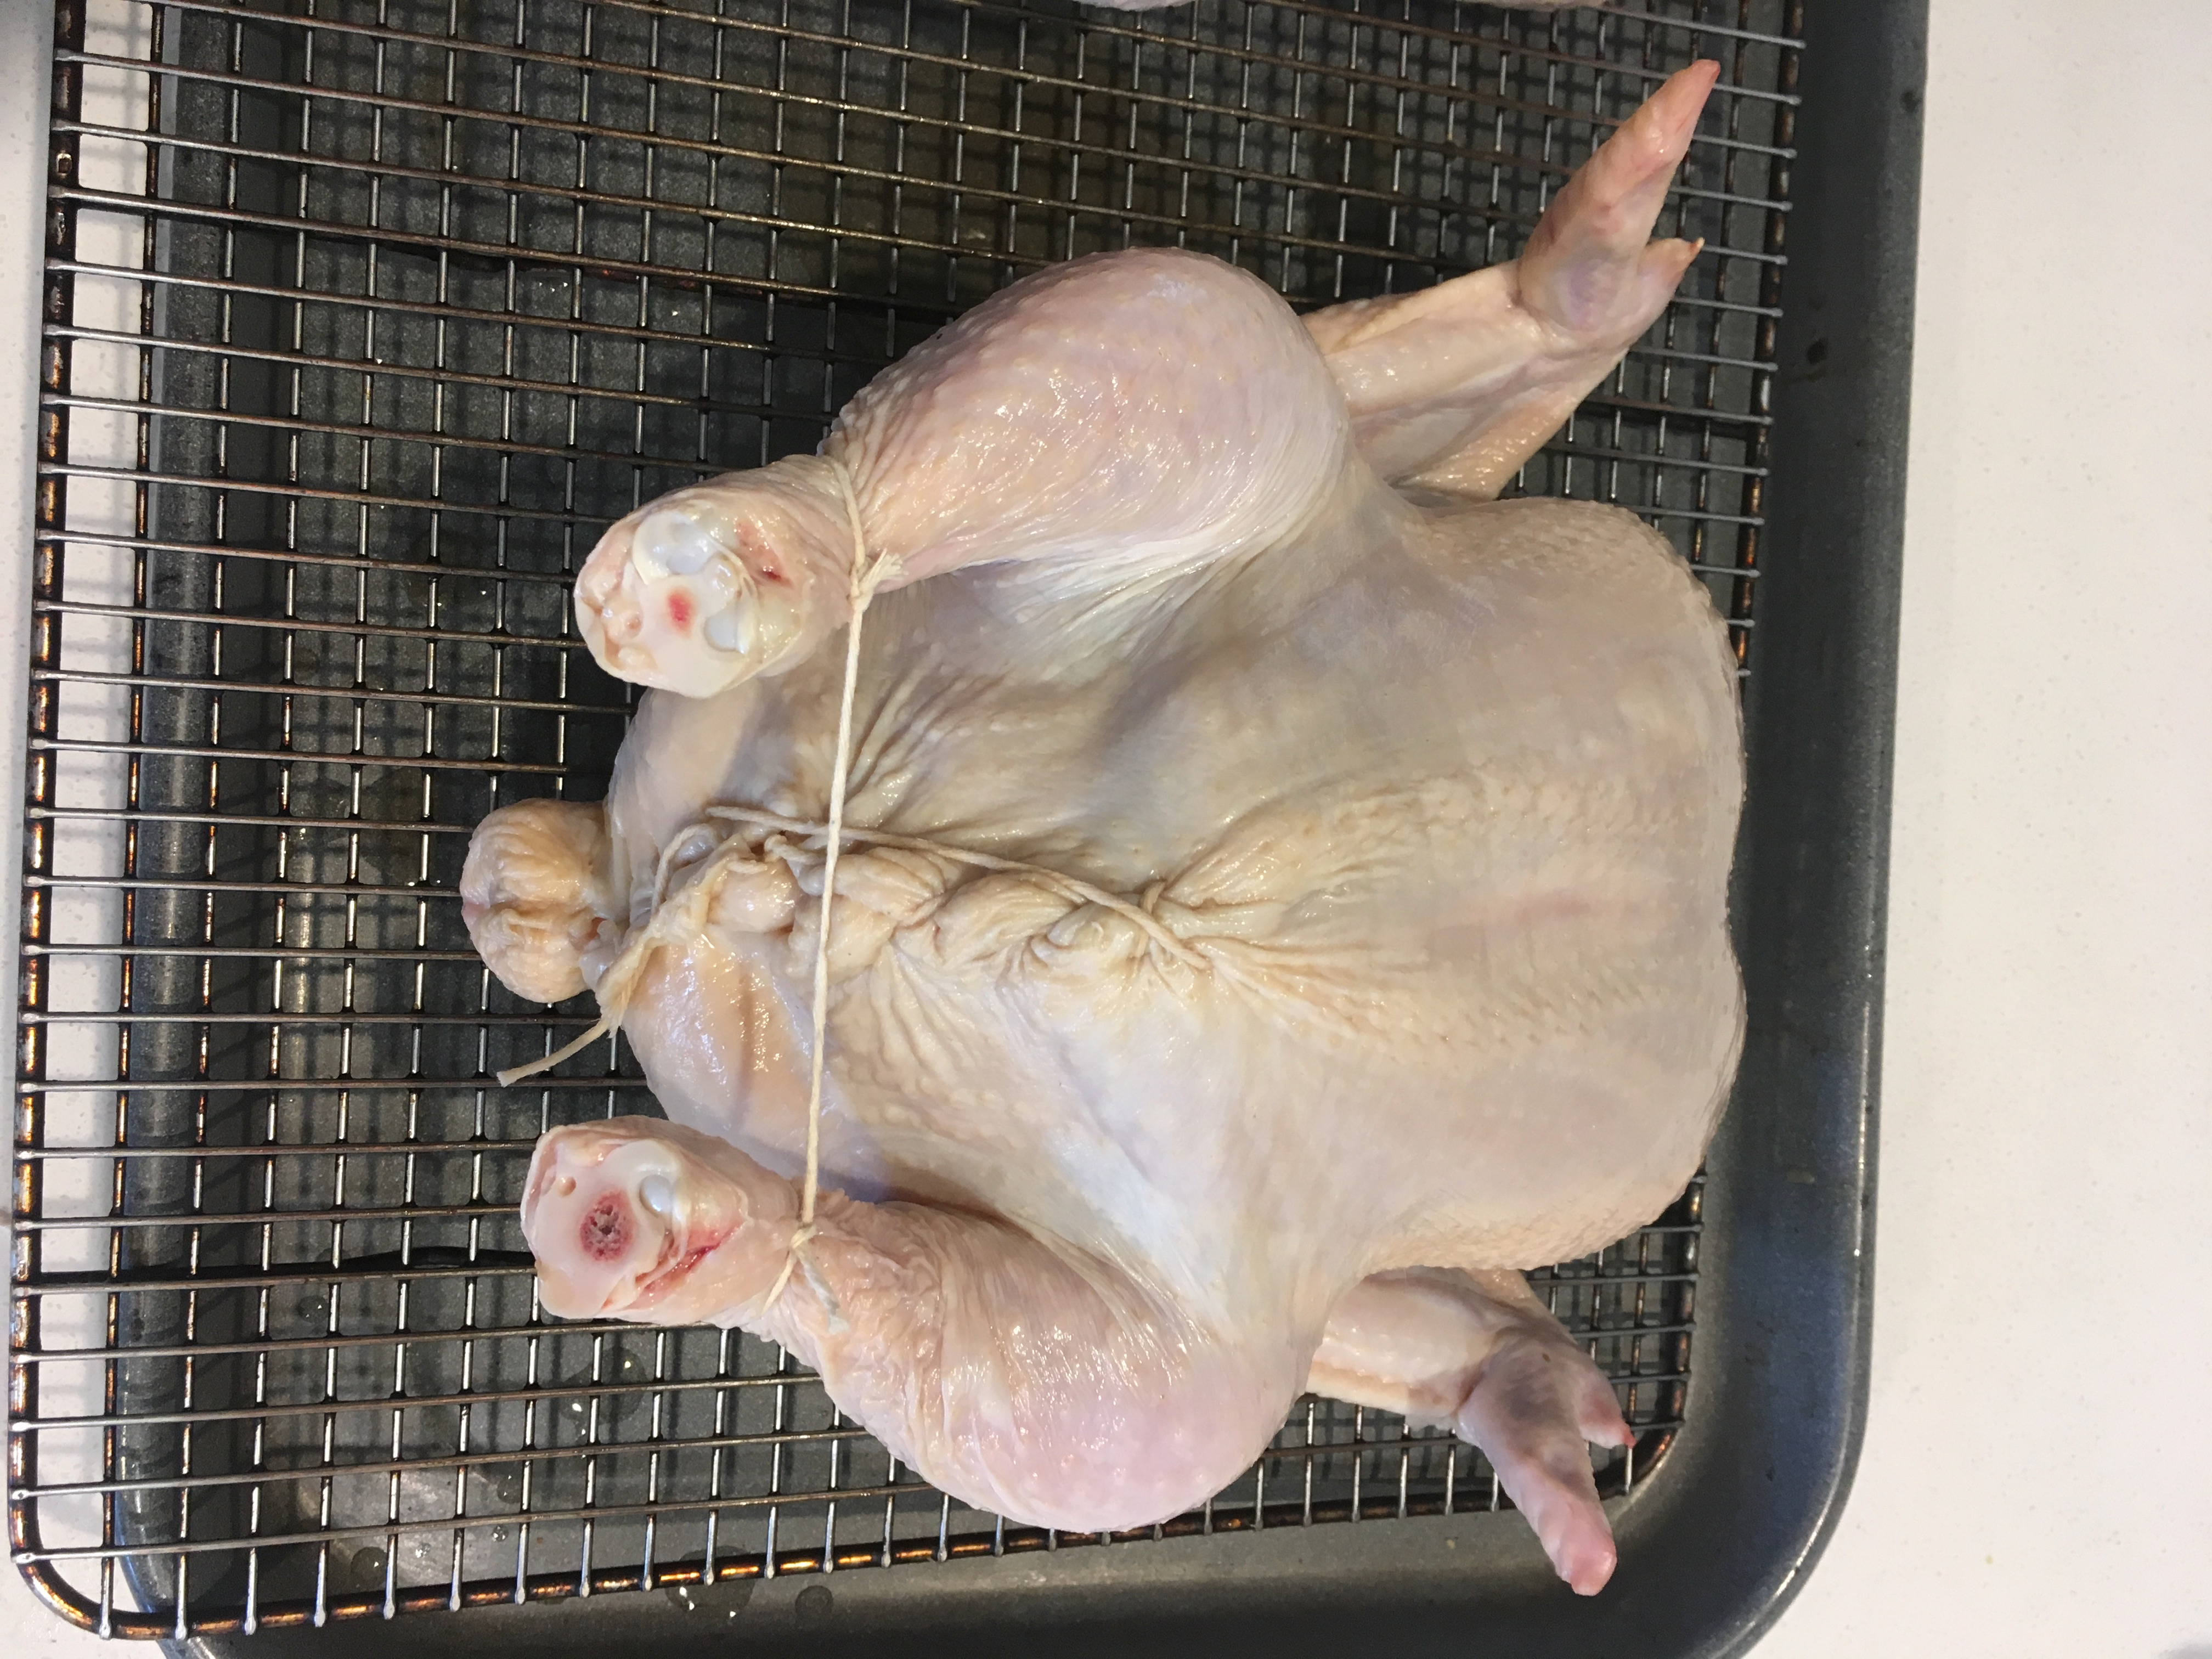
\includegraphics[width=0.25\textwidth]{\imageDir/\fileName/IMG_3219.jpg} \\
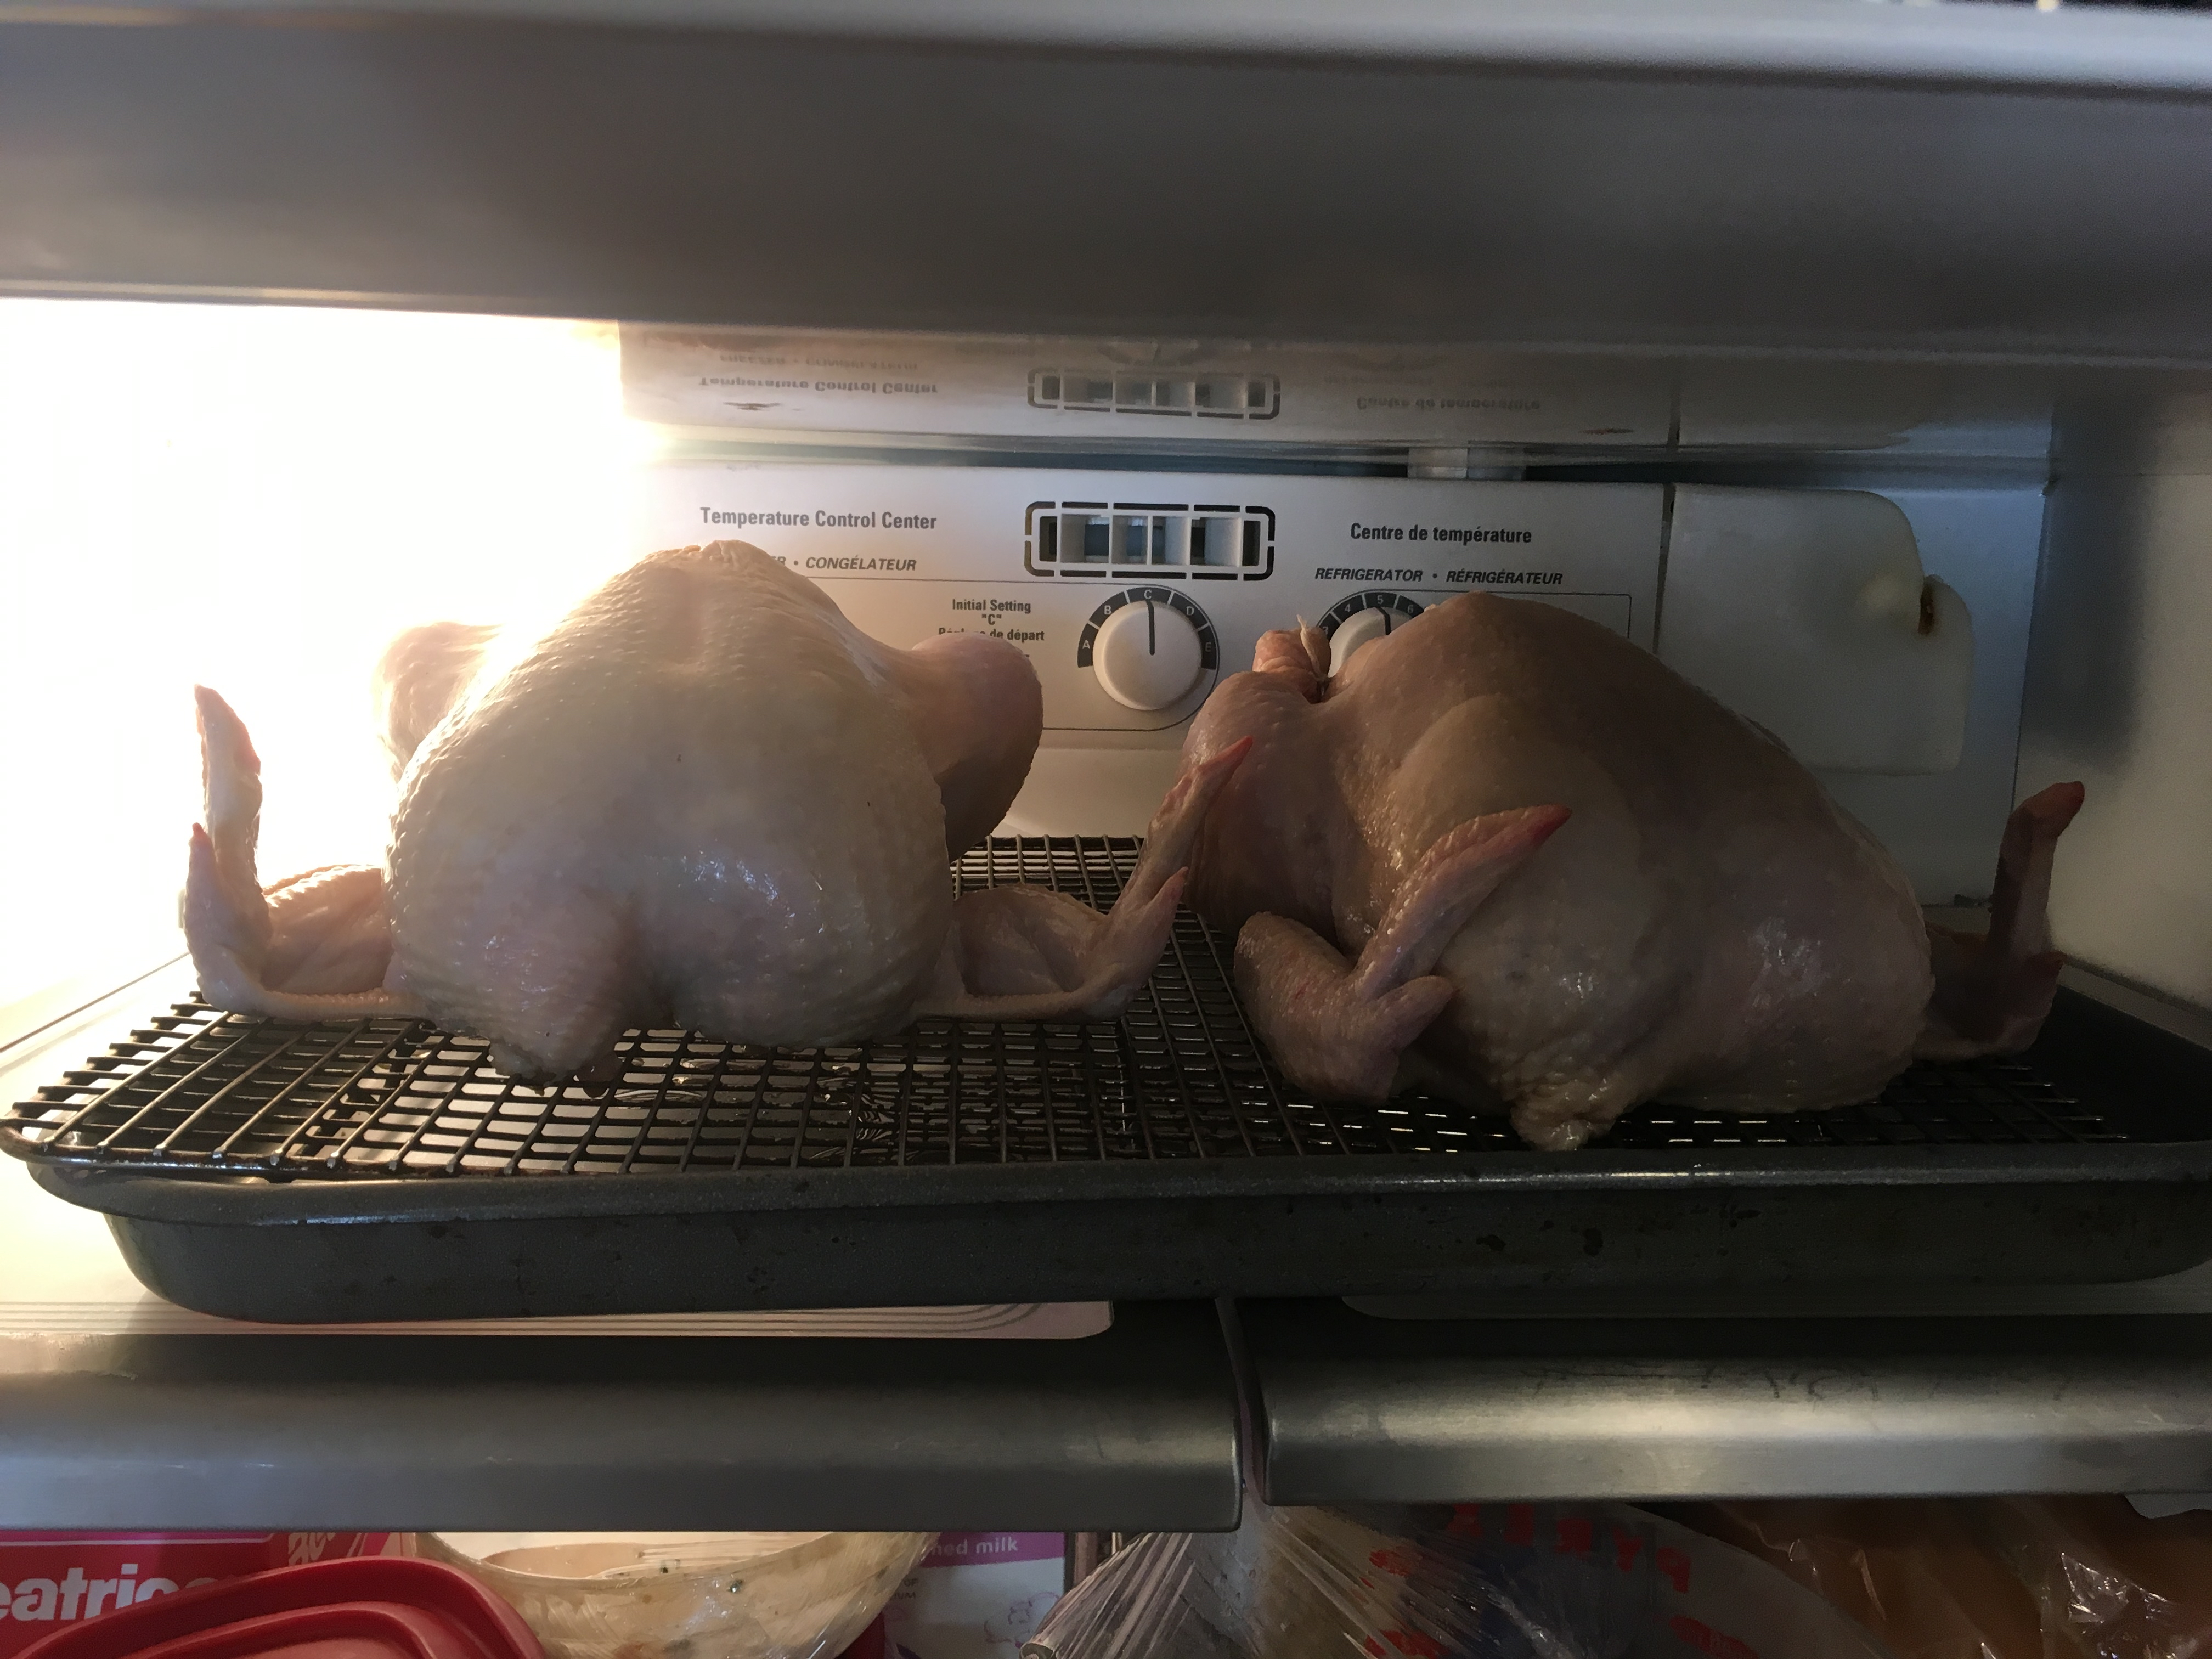
\includegraphics[width=0.25\textwidth]{\imageDir/\fileName/IMG_3220.jpg} &
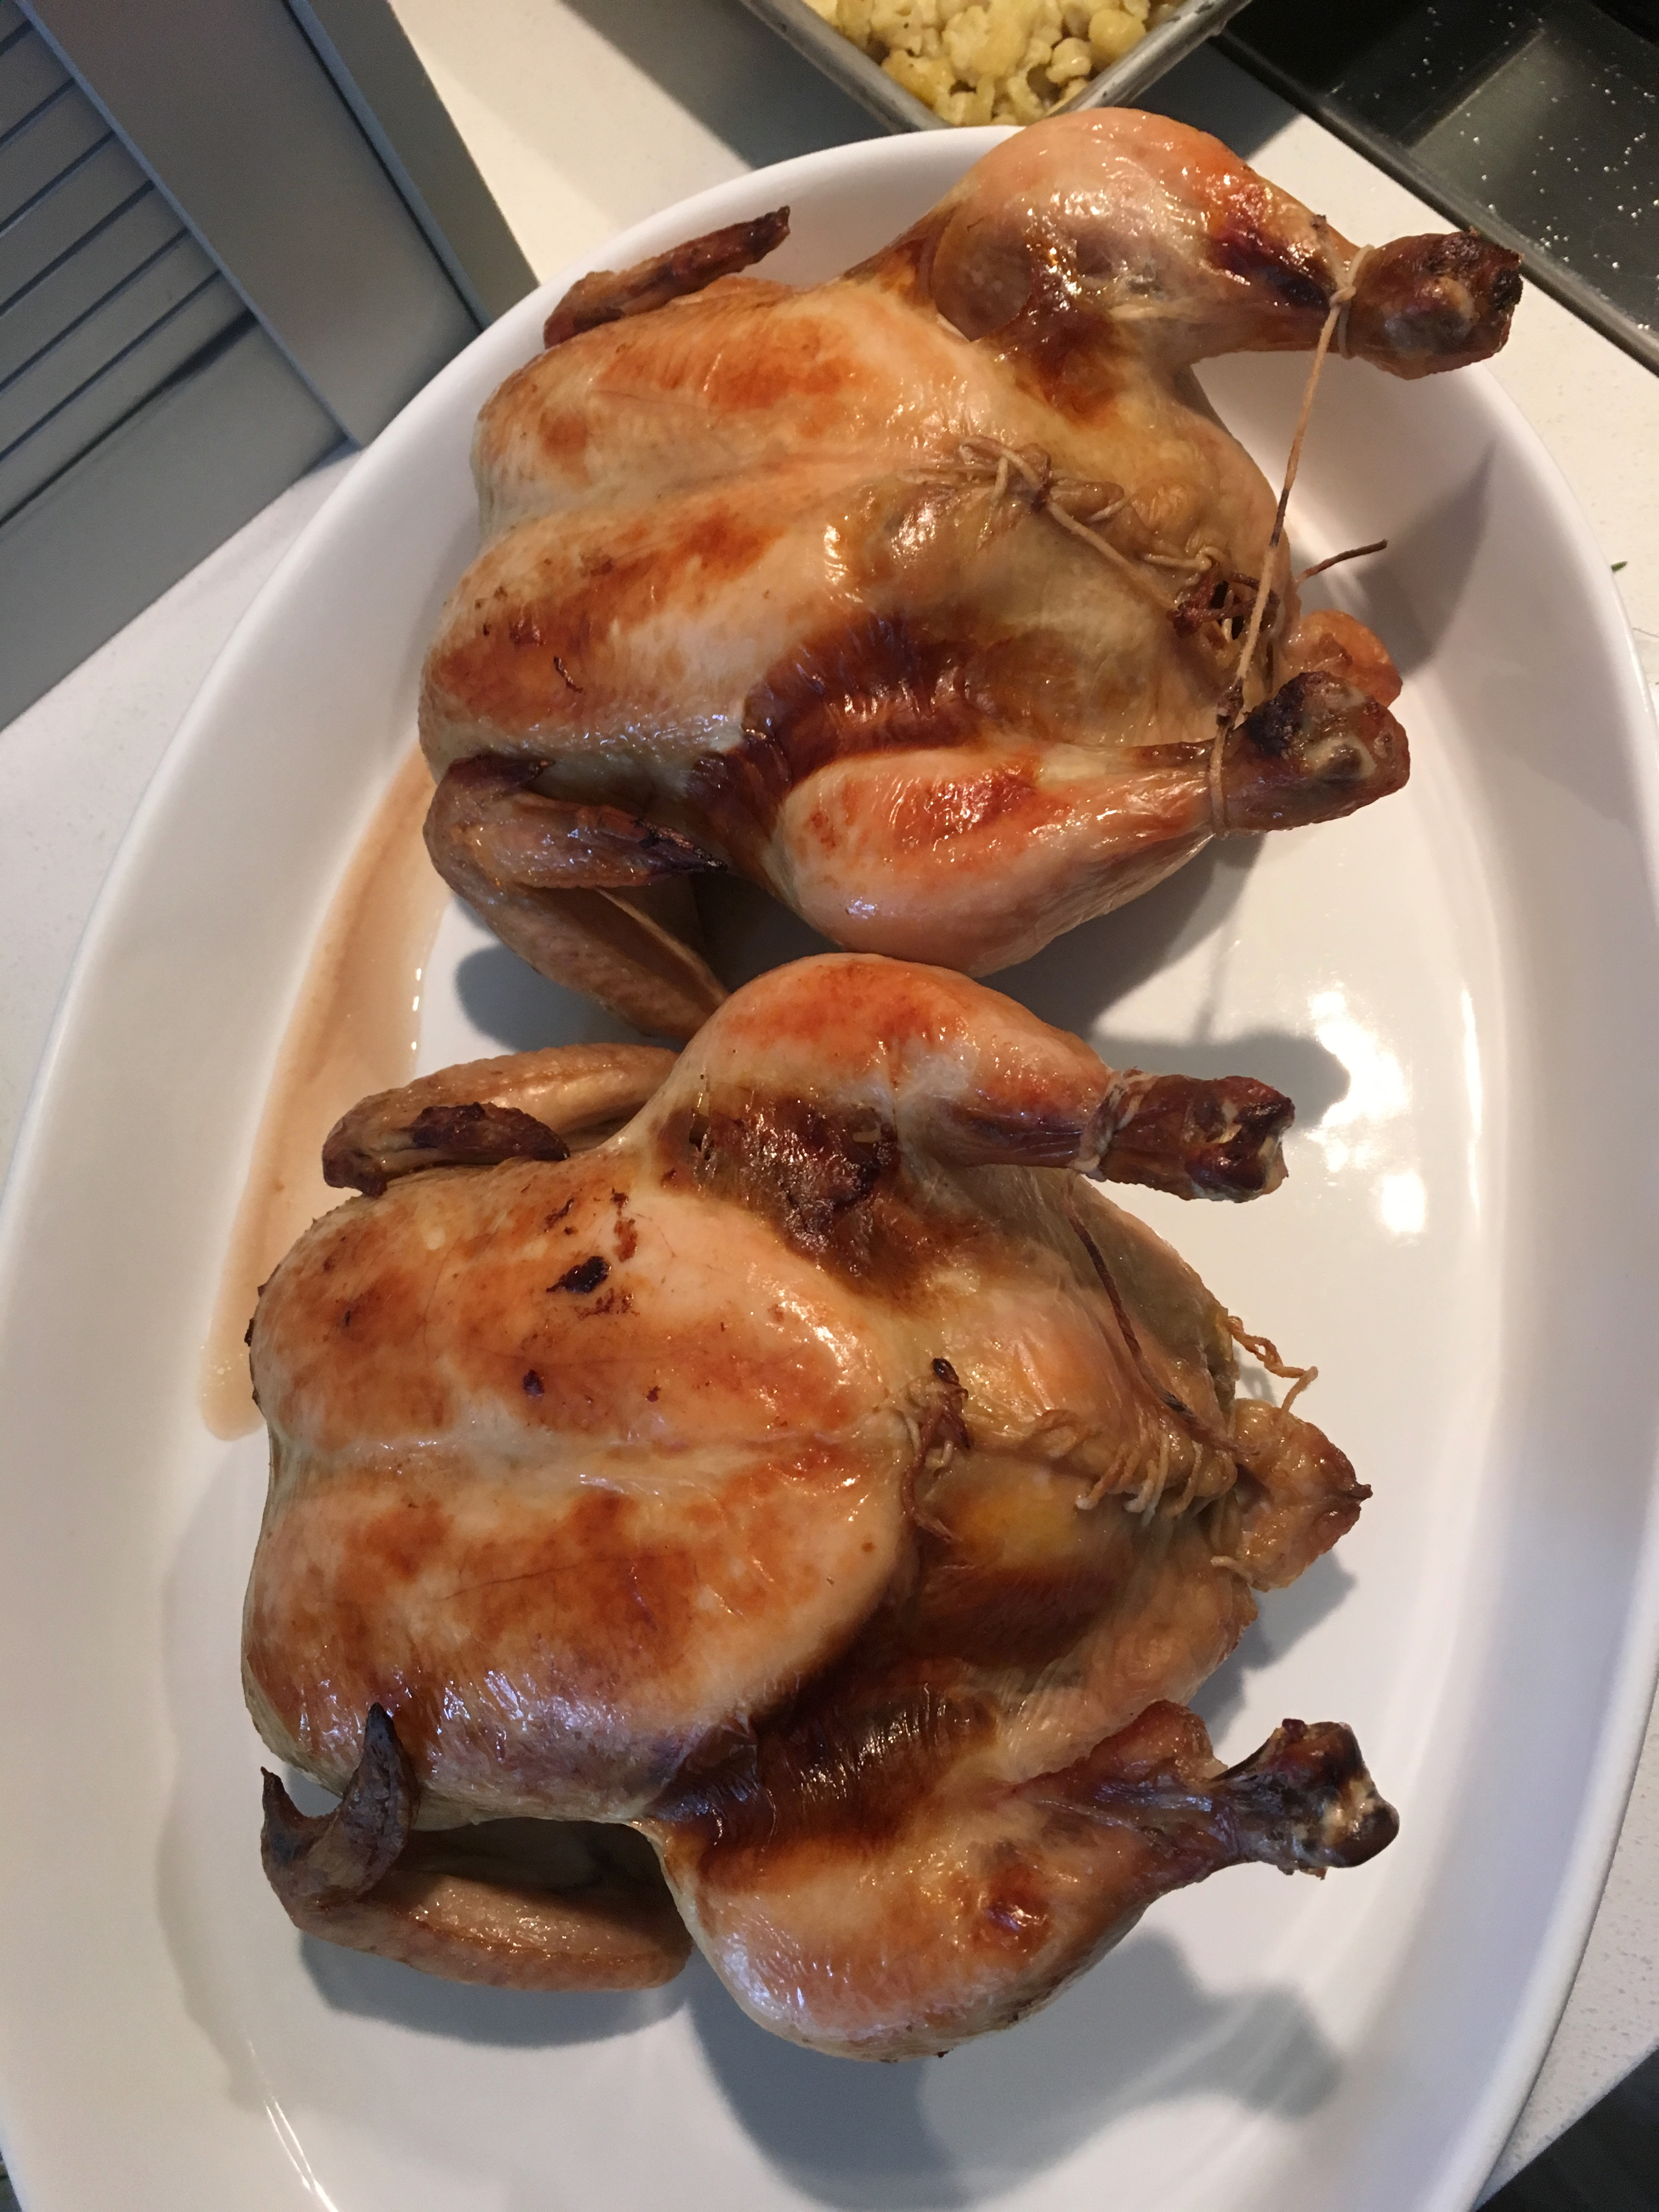
\includegraphics[width=0.25\textwidth]{\imageDir/\fileName/IMG_3228.jpg} \\
\end{tabular}
\end{table}


\end{document}




